\hypertarget{_tsyg2004_8c}{
\section{/home/mgh/LanlGeoMag/libLanlGeoMag/Tsyg2004.c File Reference}
\label{_tsyg2004_8c}\index{/home/mgh/LanlGeoMag/libLanlGeoMag/Tsyg2004.c@{/home/mgh/LanlGeoMag/libLanlGeoMag/Tsyg2004.c}}
}
{\tt \#include $<$stdio.h$>$}\par
{\tt \#include $<$stdlib.h$>$}\par
{\tt \#include $<$math.h$>$}\par


Include dependency graph for Tsyg2004.c:\nopagebreak
\begin{figure}[H]
\begin{center}
\leavevmode
\includegraphics[width=143pt]{_tsyg2004_8c__incl}
\end{center}
\end{figure}
\subsection*{Data Structures}
\begin{CompactItemize}
\item 
struct \hyperlink{struct___c_b___t_a_i_l}{\_\-CB\_\-TAIL}
\item 
struct \hyperlink{struct___c_b___b_i_r_k_p_a_r}{\_\-CB\_\-BIRKPAR}
\item 
struct \hyperlink{struct___c_b___r_c_p_a_r}{\_\-CB\_\-RCPAR}
\item 
struct \hyperlink{struct___c_b___g}{\_\-CB\_\-G}
\item 
struct \hyperlink{struct___c_b___r_h0}{\_\-CB\_\-RH0}
\item 
struct \hyperlink{struct___c_b___d_p_h_i___b___r_h_o0}{\_\-CB\_\-DPHI\_\-B\_\-RHO0}
\item 
struct \hyperlink{struct___c_b___m_o_d_e_n_u_m}{\_\-CB\_\-MODENUM}
\item 
struct \hyperlink{struct___c_b___d_t_h_e_t_a}{\_\-CB\_\-DTHETA}
\item 
struct \hyperlink{struct___t_s04_info}{\_\-TS04Info}
\end{CompactItemize}
\subsection*{Defines}
\begin{CompactItemize}
\item 
\#define \hyperlink{_tsyg2004_8c_a8cecfc5c5c054d2875c03e77b7be15d}{TRUE}~1
\item 
\#define \hyperlink{_tsyg2004_8c_a93f0eb578d23995850d61f7d61c55c1}{FALSE}~0
\end{CompactItemize}
\subsection*{Functions}
\begin{CompactItemize}
\item 
void \hyperlink{_tsyg2004_8c_5c047252d169aae0974e5bfed6d71085}{Lgm\_\-EXTERN} (int IOPGEN, int IOPT, int IOPB, int IOPR, double $\ast$A, int NTOT, double PDYN, double DST, double BXIMF, double BYIMF, double BZIMF, double W1, double W2, double W3, double W4, double W5, double W6, double PS, double X, double Y, double Z, double $\ast$BXCF, double $\ast$BYCF, double $\ast$BZCF, double $\ast$BXT1, double $\ast$BYT1, double $\ast$BZT1, double $\ast$BXT2, double $\ast$BYT2, double $\ast$BZT2, double $\ast$BXSRC, double $\ast$BYSRC, double $\ast$BZSRC, double $\ast$BXPRC, double $\ast$BYPRC, double $\ast$BZPRC, double $\ast$BXR11, double $\ast$BYR11, double $\ast$BZR11, double $\ast$BXR12, double $\ast$BYR12, double $\ast$BZR12, double $\ast$BXR21, double $\ast$BYR21, double $\ast$BZR21, double $\ast$BXR22, double $\ast$BYR22, double $\ast$BZR22, double $\ast$HXIMF, double $\ast$HYIMF, double $\ast$HZIMF, double $\ast$BBX, double $\ast$BBY, double $\ast$BBZ)
\item 
void \hyperlink{_tsyg2004_8c_464f1d83937f8412873a74ee415058a4}{SHLCAR3X3} (double X, double Y, double Z, double PS, double $\ast$BX, double $\ast$BY, double $\ast$BZ)
\item 
void \hyperlink{_tsyg2004_8c_3ec00913121c60795f4052645698ddba}{DEFORMED} (int IOPT, double PS, double X, double Y, double Z, double $\ast$BX1, double $\ast$BY1, double $\ast$BZ1, double $\ast$BX2, double $\ast$BY2, double $\ast$BZ2)
\item 
void \hyperlink{_tsyg2004_8c_584f134348f99945741cf42bfbd511d5}{WARPED} (int IOPT, double PS, double X, double Y, double Z, double $\ast$BX1, double $\ast$BY1, double $\ast$BZ1, double $\ast$BX2, double $\ast$BY2, double $\ast$BZ2)
\item 
void \hyperlink{_tsyg2004_8c_9114d15d3eb4beb81639e71c0b0235dd}{UNWARPED} (int IOPT, double X, double Y, double Z, double $\ast$BX1, double $\ast$BY1, double $\ast$BZ1, double $\ast$BX2, double $\ast$BY2, double $\ast$BZ2)
\item 
void \hyperlink{_tsyg2004_8c_81b0851907208b45c9721ef40e1e37a3}{TAILDISK} (double D0, double DELTADX, double DELTADY, double X, double Y, double Z, double $\ast$BX, double $\ast$BY, double $\ast$BZ)
\item 
void \hyperlink{_tsyg2004_8c_d52c3a08bf2c11b9784a6ce1eb480fed}{SHLCAR5X5} (double $\ast$A, double X, double Y, double Z, double DSHIFT, double $\ast$HX, double $\ast$HY, double $\ast$HZ)
\item 
void \hyperlink{_tsyg2004_8c_a448f7ca5c043203dab6208c5c982571}{BIRK\_\-TOT} (int IOPB, double PS, double X, double Y, double Z, double $\ast$BX11, double $\ast$BY11, double $\ast$BZ11, double $\ast$BX12, double $\ast$BY12, double $\ast$BZ12, double $\ast$BX21, double $\ast$BY21, double $\ast$BZ21, double $\ast$BX22, double $\ast$BY22, double $\ast$BZ22)
\item 
void \hyperlink{_tsyg2004_8c_05b3a8c8d1e1b62725abe895df3d1ca1}{BIRK\_\-1N2} (int NUMB, int MODE, double PS, double X, double Y, double Z, double $\ast$BX, double $\ast$BY, double $\ast$BZ)
\item 
void \hyperlink{_tsyg2004_8c_b05c2844104041ea55de4c30aaa5b968}{TWOCONES} (double $\ast$A, double X, double Y, double Z, double $\ast$BX, double $\ast$BY, double $\ast$BZ)
\item 
void \hyperlink{_tsyg2004_8c_d3ff91c1de1106c25ccbf3c1694cc883}{ONE\_\-CONE} (double $\ast$A, double X, double Y, double Z, double $\ast$BX, double $\ast$BY, double $\ast$BZ)
\item 
double \hyperlink{_tsyg2004_8c_af80d04276fc0dce8abc24392512cf8e}{THETA\_\-S} (double $\ast$A, double R, double THETA)
\item 
double \hyperlink{_tsyg2004_8c_22701b7ad2e702887750fdec469f01fb}{R\_\-S} (double $\ast$A, double R, double THETA)
\item 
void \hyperlink{_tsyg2004_8c_8e93acc99263e229c4b81a6c4cd9f148}{FIALCOS} (double R, double THETA, double PHI, double $\ast$BTHETA, double $\ast$BPHI, int N, double THETA0, double DT)
\item 
void \hyperlink{_tsyg2004_8c_723d4ced4ac10c32344d63bda6126fdf}{BIRK\_\-SHL} (int, int, int, int, int, double $\ast$A, double PS, double X\_\-SC, double X, double Y, double Z, double $\ast$BX, double $\ast$BY, double $\ast$BZ)
\item 
void \hyperlink{_tsyg2004_8c_2a492ba836369d99dfb597c1675f6a33}{FULL\_\-RC} (int IOPR, double PS, double X, double Y, double Z, double $\ast$BXSRC, double $\ast$BYSRC, double $\ast$BZSRC, double $\ast$BXPRC, double $\ast$BYPRC, double $\ast$BZPRC)
\item 
void \hyperlink{_tsyg2004_8c_9d8e16b4209da2c6896cb9fb1531f2fa}{SRC\_\-PRC} (int IOPR, double SC\_\-SY, double SC\_\-PR, double PHI, double PS, double X, double Y, double Z, double $\ast$BXSRC, double $\ast$BYSRC, double $\ast$BZSRC, double $\ast$BXPRC, double $\ast$BYPRC, double $\ast$BZPRC)
\item 
void \hyperlink{_tsyg2004_8c_16ec50640c104c5c2a57ef6a51b21f01}{RC\_\-SYMM} (double X, double Y, double Z, double $\ast$BX, double $\ast$BY, double $\ast$BZ)
\item 
double \hyperlink{_tsyg2004_8c_55f2b5b45100a3e191f3423e007d7174}{AP} (double R, double SINT, double COST)
\item 
void \hyperlink{_tsyg2004_8c_a49661b45ed199138df07d1806ad7240}{PRC\_\-SYMM} (double X, double Y, double Z, double $\ast$BX, double $\ast$BY, double $\ast$BZ)
\item 
double \hyperlink{_tsyg2004_8c_184ae8e5e4f65974829d3ff56683be12}{APPRC} (double R, double SINT, double COST)
\item 
void \hyperlink{_tsyg2004_8c_7d3132f7a6ed31b467740063133da1fe}{PRC\_\-QUAD} (double X, double Y, double Z, double $\ast$BX, double $\ast$BY, double $\ast$BZ)
\item 
double \hyperlink{_tsyg2004_8c_51ea88e5a0772dd9763092b23868d83e}{BR\_\-PRC\_\-Q} (double R, double SINT, double COST)
\item 
double \hyperlink{_tsyg2004_8c_40293e54c4b1290d9463ec556292303b}{BT\_\-PRC\_\-Q} (double R, double SINT, double COST)
\item 
void \hyperlink{_tsyg2004_8c_e9137c27c3c66aef974f6c4017b6ab9d}{FFS} (double A, double A0, double DA, double $\ast$F, double $\ast$FA, double $\ast$FS)
\item 
void \hyperlink{_tsyg2004_8c_ae1fabae2232fcfa073907bc921dbf66}{RC\_\-SHIELD} (double $\ast$A, double PS, double X\_\-SC, double X, double Y, double Z, double $\ast$BX, double $\ast$BY, double $\ast$BZ)
\item 
void \hyperlink{_tsyg2004_8c_b1ff14f59abcc09994d8743db9a8f736}{DIPOLE} (double PS, double X, double Y, double Z, double $\ast$BX, double $\ast$BY, double $\ast$BZ)
\item 
\hyperlink{struct___t_s04_info}{\_\-TS04Info} $\ast$ \hyperlink{_tsyg2004_8c_2a5550ebc6d255713c18b87010ed2594}{init\_\-TS04Info} ()
\item 
void \hyperlink{_tsyg2004_8c_54ecb238c46c4acfe5e022e19cc326ec}{Lgm\_\-T04\_\-s} (int IOPT, double $\ast$PARMOD, double PS, double SINPS, double COSPS, double X, double Y, double Z, double $\ast$BX, double $\ast$BY, double $\ast$BZ)
\end{CompactItemize}
\subsection*{Variables}
\begin{CompactItemize}
\item 
double \hyperlink{_tsyg2004_8c_5b35fcda1a15310fa7b7e3e242431de3}{sin\_\-psi}
\item 
double \hyperlink{_tsyg2004_8c_98e0e08bb8a65f90813e5adb482aeb2c}{cos\_\-psi}
\end{CompactItemize}


\subsection{Define Documentation}
\hypertarget{_tsyg2004_8c_a8cecfc5c5c054d2875c03e77b7be15d}{
\index{Tsyg2004.c@{Tsyg2004.c}!TRUE@{TRUE}}
\index{TRUE@{TRUE}!Tsyg2004.c@{Tsyg2004.c}}
\subsubsection[{TRUE}]{\setlength{\rightskip}{0pt plus 5cm}\#define TRUE~1}}
\label{_tsyg2004_8c_a8cecfc5c5c054d2875c03e77b7be15d}




Definition at line 10 of file Tsyg2004.c.\hypertarget{_tsyg2004_8c_a93f0eb578d23995850d61f7d61c55c1}{
\index{Tsyg2004.c@{Tsyg2004.c}!FALSE@{FALSE}}
\index{FALSE@{FALSE}!Tsyg2004.c@{Tsyg2004.c}}
\subsubsection[{FALSE}]{\setlength{\rightskip}{0pt plus 5cm}\#define FALSE~0}}
\label{_tsyg2004_8c_a93f0eb578d23995850d61f7d61c55c1}




Definition at line 11 of file Tsyg2004.c.

\subsection{Function Documentation}
\hypertarget{_tsyg2004_8c_5c047252d169aae0974e5bfed6d71085}{
\index{Tsyg2004.c@{Tsyg2004.c}!Lgm\_\-EXTERN@{Lgm\_\-EXTERN}}
\index{Lgm\_\-EXTERN@{Lgm\_\-EXTERN}!Tsyg2004.c@{Tsyg2004.c}}
\subsubsection[{Lgm\_\-EXTERN}]{\setlength{\rightskip}{0pt plus 5cm}void Lgm\_\-EXTERN (int {\em IOPGEN}, \/  int {\em IOPT}, \/  int {\em IOPB}, \/  int {\em IOPR}, \/  double $\ast$ {\em A}, \/  int {\em NTOT}, \/  double {\em PDYN}, \/  double {\em DST}, \/  double {\em BXIMF}, \/  double {\em BYIMF}, \/  double {\em BZIMF}, \/  double {\em W1}, \/  double {\em W2}, \/  double {\em W3}, \/  double {\em W4}, \/  double {\em W5}, \/  double {\em W6}, \/  double {\em PS}, \/  double {\em X}, \/  double {\em Y}, \/  double {\em Z}, \/  double $\ast$ {\em BXCF}, \/  double $\ast$ {\em BYCF}, \/  double $\ast$ {\em BZCF}, \/  double $\ast$ {\em BXT1}, \/  double $\ast$ {\em BYT1}, \/  double $\ast$ {\em BZT1}, \/  double $\ast$ {\em BXT2}, \/  double $\ast$ {\em BYT2}, \/  double $\ast$ {\em BZT2}, \/  double $\ast$ {\em BXSRC}, \/  double $\ast$ {\em BYSRC}, \/  double $\ast$ {\em BZSRC}, \/  double $\ast$ {\em BXPRC}, \/  double $\ast$ {\em BYPRC}, \/  double $\ast$ {\em BZPRC}, \/  double $\ast$ {\em BXR11}, \/  double $\ast$ {\em BYR11}, \/  double $\ast$ {\em BZR11}, \/  double $\ast$ {\em BXR12}, \/  double $\ast$ {\em BYR12}, \/  double $\ast$ {\em BZR12}, \/  double $\ast$ {\em BXR21}, \/  double $\ast$ {\em BYR21}, \/  double $\ast$ {\em BZR21}, \/  double $\ast$ {\em BXR22}, \/  double $\ast$ {\em BYR22}, \/  double $\ast$ {\em BZR22}, \/  double $\ast$ {\em HXIMF}, \/  double $\ast$ {\em HYIMF}, \/  double $\ast$ {\em HZIMF}, \/  double $\ast$ {\em BBX}, \/  double $\ast$ {\em BBY}, \/  double $\ast$ {\em BBZ})}}
\label{_tsyg2004_8c_5c047252d169aae0974e5bfed6d71085}


\hypertarget{_tsyg2004_8c_464f1d83937f8412873a74ee415058a4}{
\index{Tsyg2004.c@{Tsyg2004.c}!SHLCAR3X3@{SHLCAR3X3}}
\index{SHLCAR3X3@{SHLCAR3X3}!Tsyg2004.c@{Tsyg2004.c}}
\subsubsection[{SHLCAR3X3}]{\setlength{\rightskip}{0pt plus 5cm}void SHLCAR3X3 (double {\em X}, \/  double {\em Y}, \/  double {\em Z}, \/  double {\em PS}, \/  double $\ast$ {\em BX}, \/  double $\ast$ {\em BY}, \/  double $\ast$ {\em BZ})}}
\label{_tsyg2004_8c_464f1d83937f8412873a74ee415058a4}




Definition at line 569 of file Tsyg2004.c.

Here is the caller graph for this function:\nopagebreak
\begin{figure}[H]
\begin{center}
\leavevmode
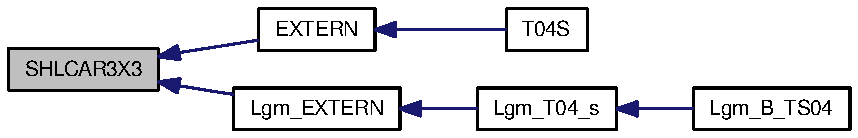
\includegraphics[width=224pt]{_tsyg2004_8c_464f1d83937f8412873a74ee415058a4_icgraph}
\end{center}
\end{figure}
\hypertarget{_tsyg2004_8c_3ec00913121c60795f4052645698ddba}{
\index{Tsyg2004.c@{Tsyg2004.c}!DEFORMED@{DEFORMED}}
\index{DEFORMED@{DEFORMED}!Tsyg2004.c@{Tsyg2004.c}}
\subsubsection[{DEFORMED}]{\setlength{\rightskip}{0pt plus 5cm}void DEFORMED (int {\em IOPT}, \/  double {\em PS}, \/  double {\em X}, \/  double {\em Y}, \/  double {\em Z}, \/  double $\ast$ {\em BX1}, \/  double $\ast$ {\em BY1}, \/  double $\ast$ {\em BZ1}, \/  double $\ast$ {\em BX2}, \/  double $\ast$ {\em BY2}, \/  double $\ast$ {\em BZ2})}}
\label{_tsyg2004_8c_3ec00913121c60795f4052645698ddba}




Definition at line 884 of file Tsyg2004.c.

Here is the call graph for this function:\nopagebreak
\begin{figure}[H]
\begin{center}
\leavevmode
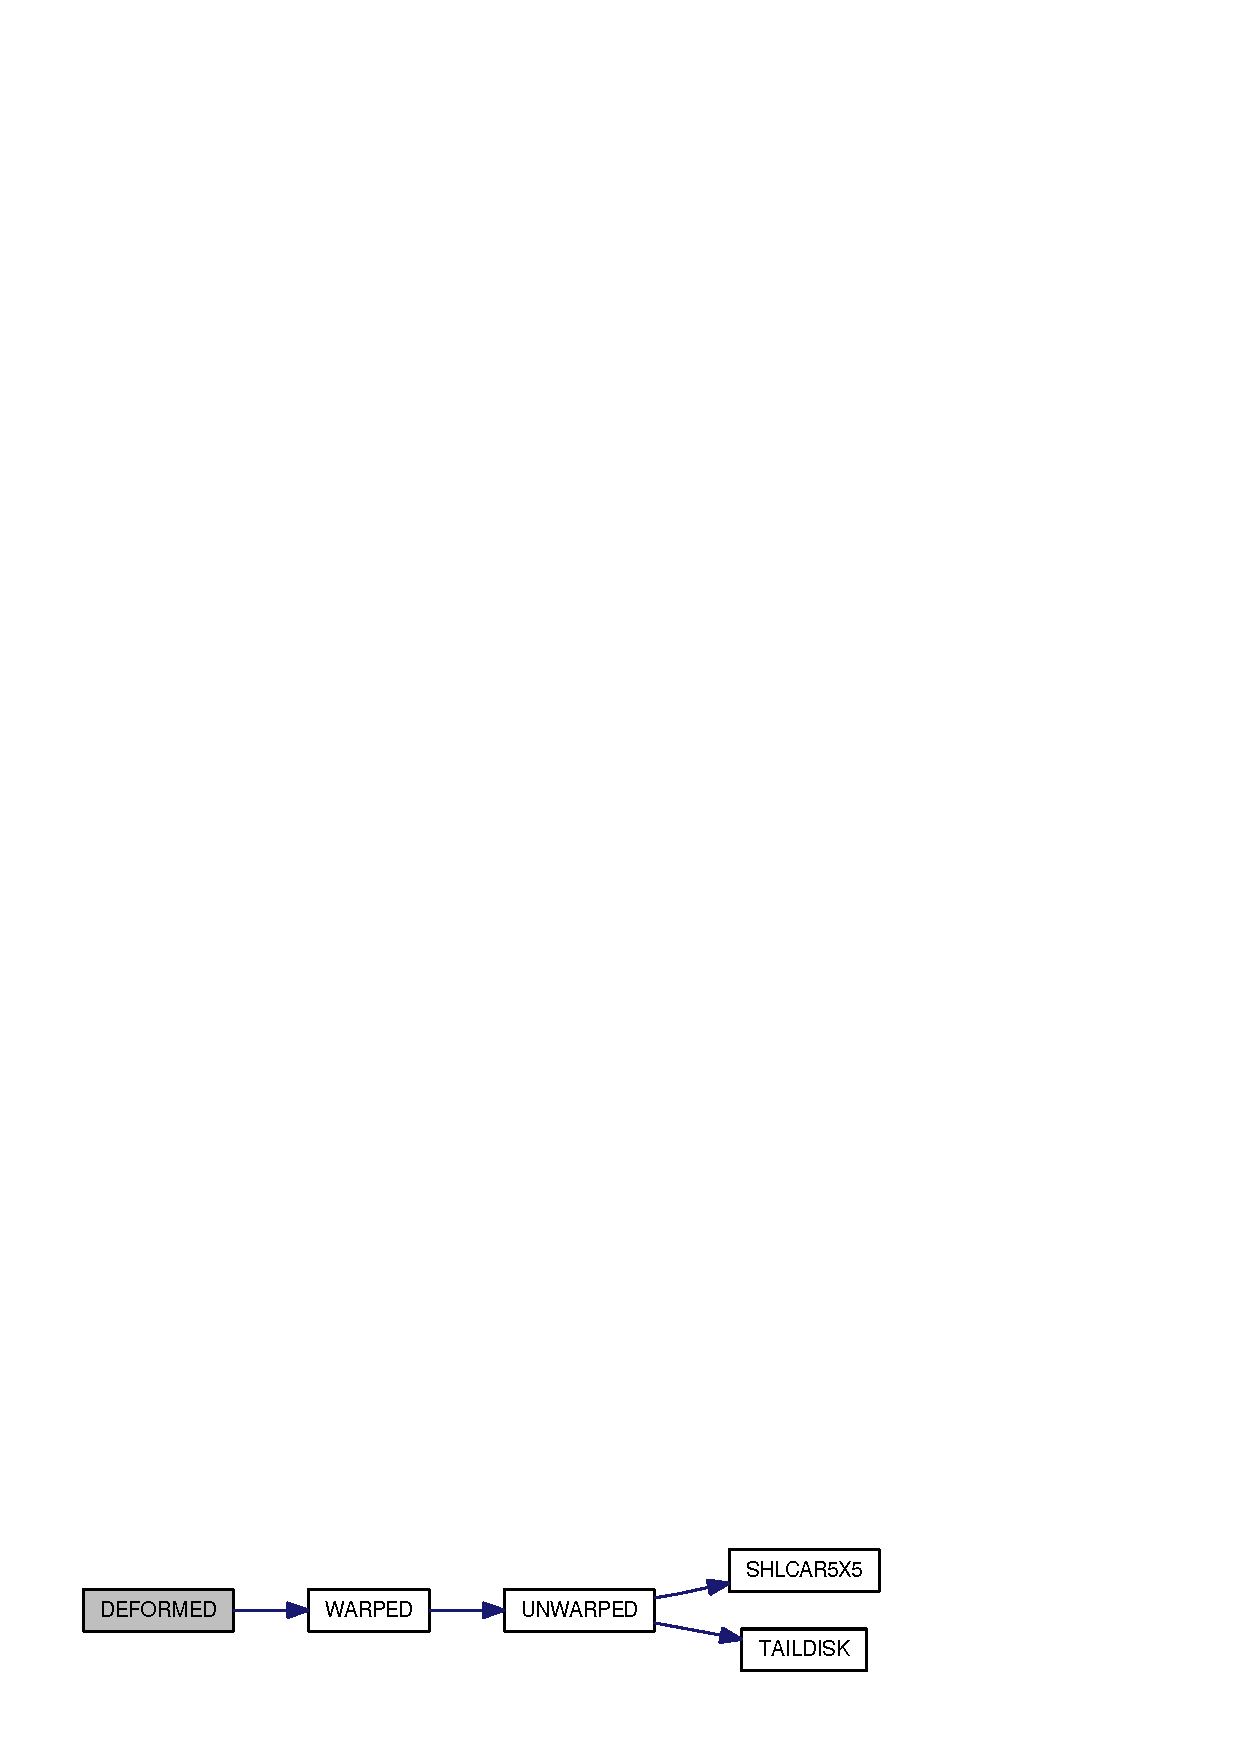
\includegraphics[width=213pt]{_tsyg2004_8c_3ec00913121c60795f4052645698ddba_cgraph}
\end{center}
\end{figure}


Here is the caller graph for this function:\nopagebreak
\begin{figure}[H]
\begin{center}
\leavevmode
\includegraphics[width=224pt]{_tsyg2004_8c_3ec00913121c60795f4052645698ddba_icgraph}
\end{center}
\end{figure}
\hypertarget{_tsyg2004_8c_584f134348f99945741cf42bfbd511d5}{
\index{Tsyg2004.c@{Tsyg2004.c}!WARPED@{WARPED}}
\index{WARPED@{WARPED}!Tsyg2004.c@{Tsyg2004.c}}
\subsubsection[{WARPED}]{\setlength{\rightskip}{0pt plus 5cm}void WARPED (int {\em IOPT}, \/  double {\em PS}, \/  double {\em X}, \/  double {\em Y}, \/  double {\em Z}, \/  double $\ast$ {\em BX1}, \/  double $\ast$ {\em BY1}, \/  double $\ast$ {\em BZ1}, \/  double $\ast$ {\em BX2}, \/  double $\ast$ {\em BY2}, \/  double $\ast$ {\em BZ2})}}
\label{_tsyg2004_8c_584f134348f99945741cf42bfbd511d5}




Definition at line 958 of file Tsyg2004.c.

Here is the call graph for this function:\nopagebreak
\begin{figure}[H]
\begin{center}
\leavevmode
\includegraphics[width=159pt]{_tsyg2004_8c_584f134348f99945741cf42bfbd511d5_cgraph}
\end{center}
\end{figure}


Here is the caller graph for this function:\nopagebreak
\begin{figure}[H]
\begin{center}
\leavevmode
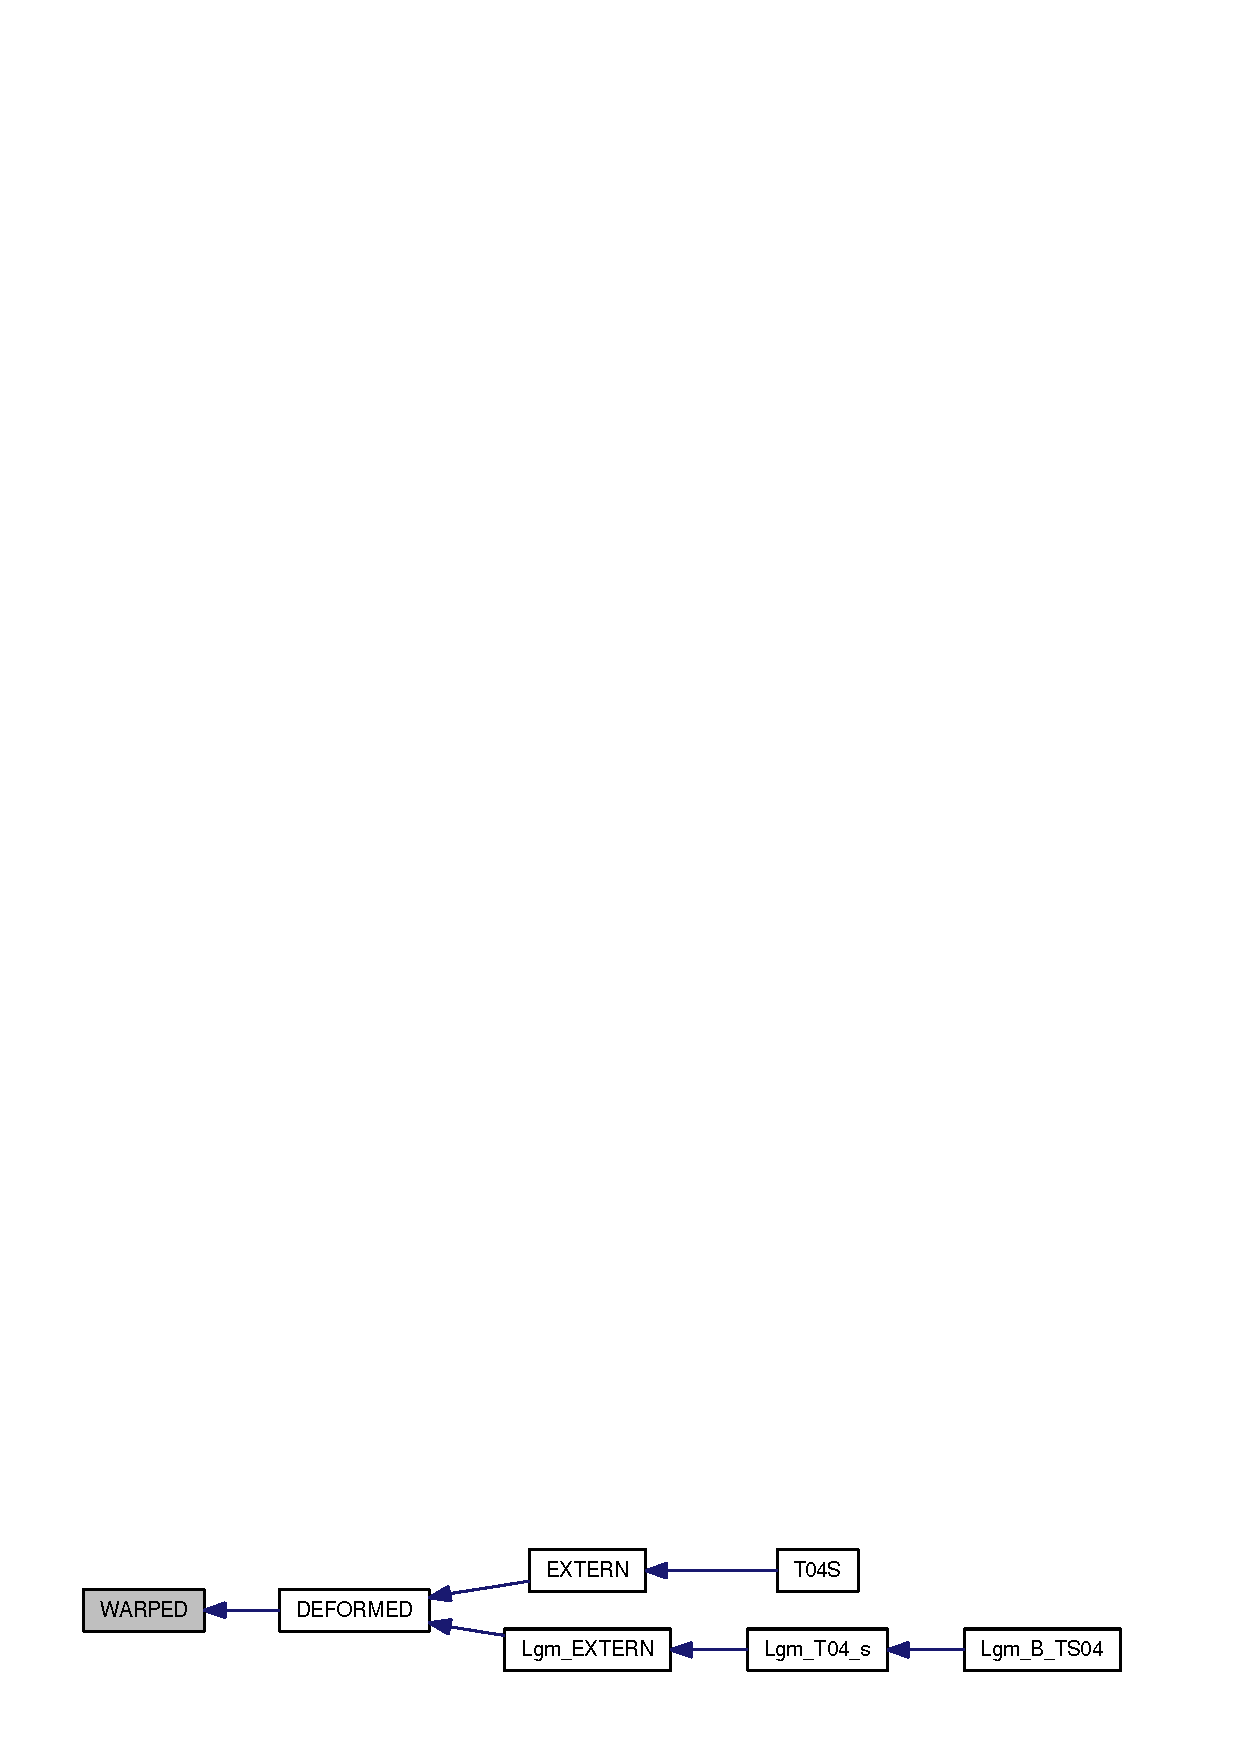
\includegraphics[width=271pt]{_tsyg2004_8c_584f134348f99945741cf42bfbd511d5_icgraph}
\end{center}
\end{figure}
\hypertarget{_tsyg2004_8c_9114d15d3eb4beb81639e71c0b0235dd}{
\index{Tsyg2004.c@{Tsyg2004.c}!UNWARPED@{UNWARPED}}
\index{UNWARPED@{UNWARPED}!Tsyg2004.c@{Tsyg2004.c}}
\subsubsection[{UNWARPED}]{\setlength{\rightskip}{0pt plus 5cm}void UNWARPED (int {\em IOPT}, \/  double {\em X}, \/  double {\em Y}, \/  double {\em Z}, \/  double $\ast$ {\em BX1}, \/  double $\ast$ {\em BY1}, \/  double $\ast$ {\em BZ1}, \/  double $\ast$ {\em BX2}, \/  double $\ast$ {\em BY2}, \/  double $\ast$ {\em BZ2})}}
\label{_tsyg2004_8c_9114d15d3eb4beb81639e71c0b0235dd}




Definition at line 1048 of file Tsyg2004.c.

Here is the call graph for this function:\nopagebreak
\begin{figure}[H]
\begin{center}
\leavevmode
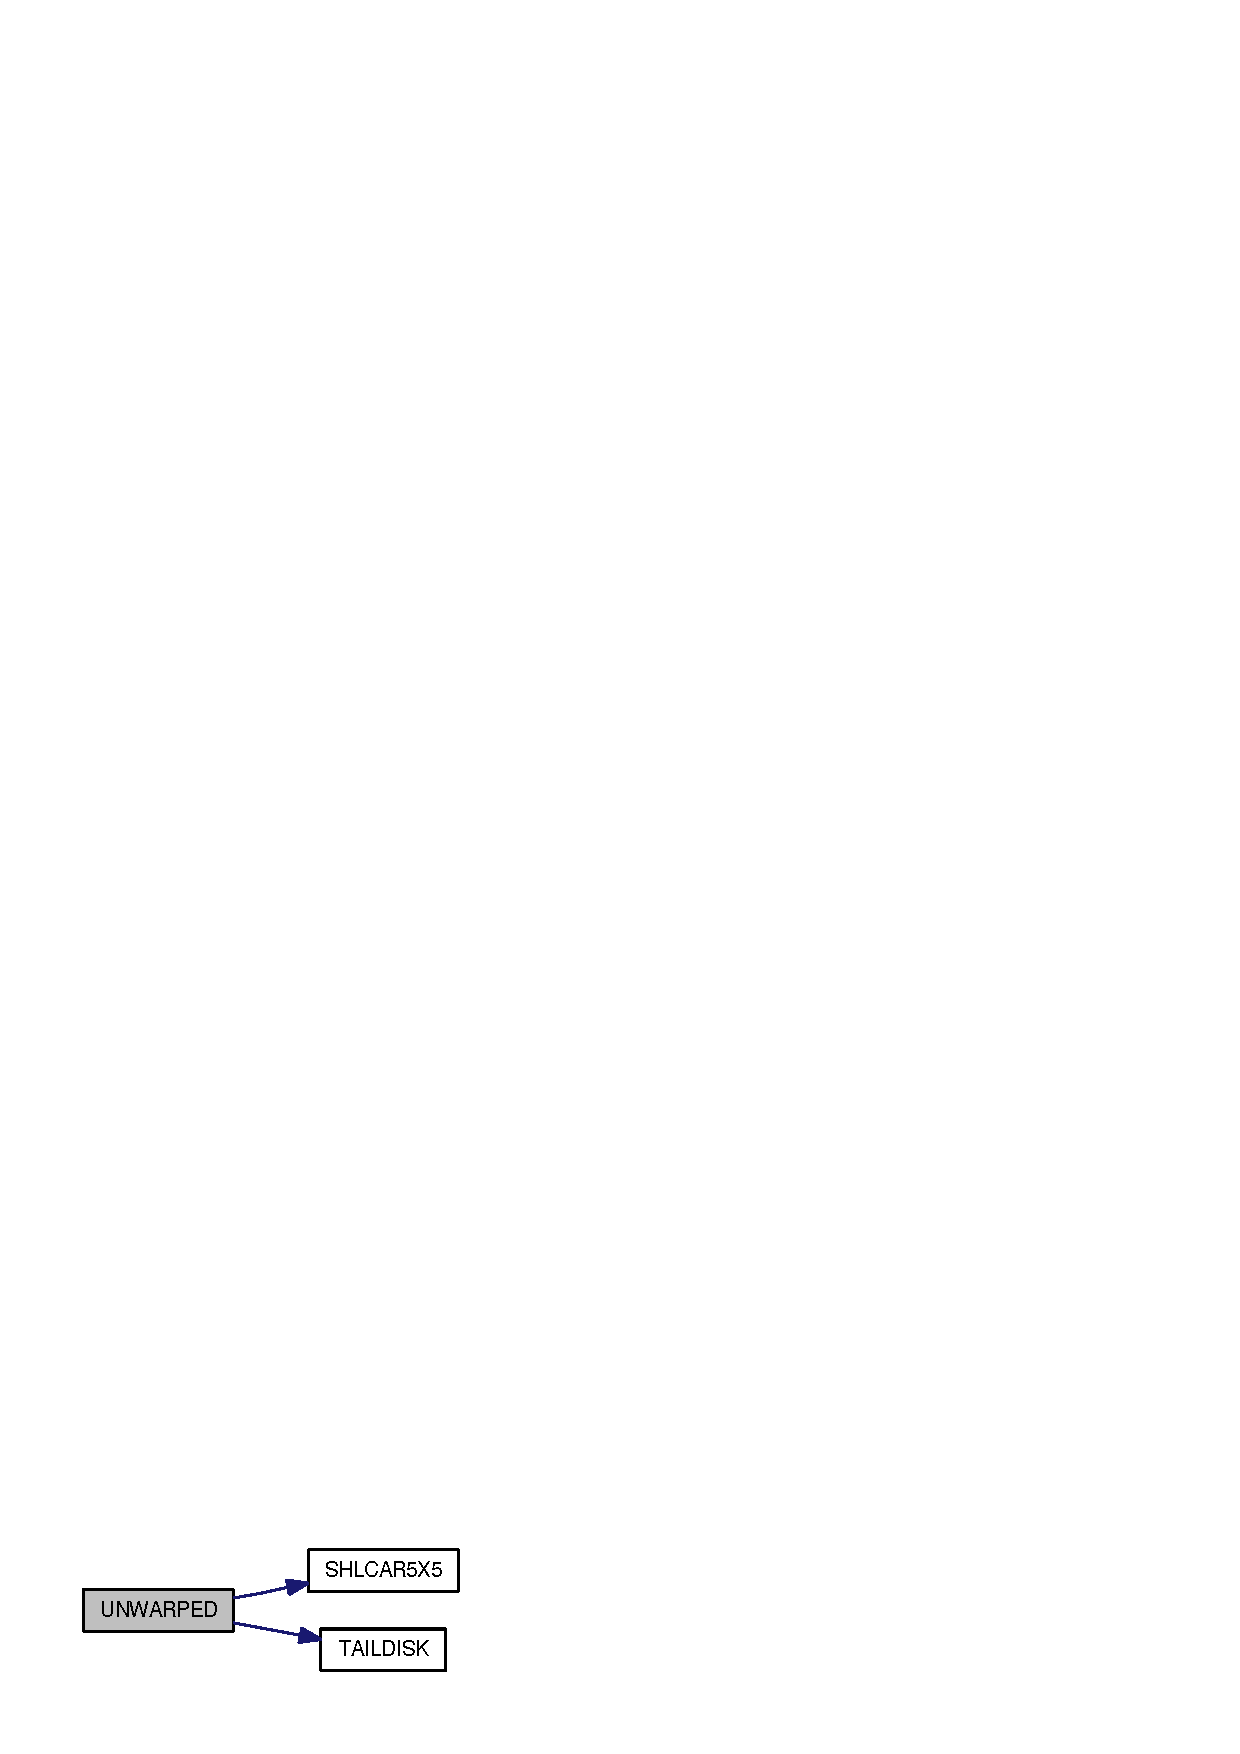
\includegraphics[width=112pt]{_tsyg2004_8c_9114d15d3eb4beb81639e71c0b0235dd_cgraph}
\end{center}
\end{figure}


Here is the caller graph for this function:\nopagebreak
\begin{figure}[H]
\begin{center}
\leavevmode
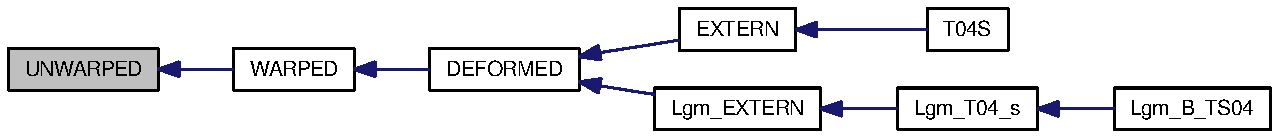
\includegraphics[width=325pt]{_tsyg2004_8c_9114d15d3eb4beb81639e71c0b0235dd_icgraph}
\end{center}
\end{figure}
\hypertarget{_tsyg2004_8c_81b0851907208b45c9721ef40e1e37a3}{
\index{Tsyg2004.c@{Tsyg2004.c}!TAILDISK@{TAILDISK}}
\index{TAILDISK@{TAILDISK}!Tsyg2004.c@{Tsyg2004.c}}
\subsubsection[{TAILDISK}]{\setlength{\rightskip}{0pt plus 5cm}void TAILDISK (double {\em D0}, \/  double {\em DELTADX}, \/  double {\em DELTADY}, \/  double {\em X}, \/  double {\em Y}, \/  double {\em Z}, \/  double $\ast$ {\em BX}, \/  double $\ast$ {\em BY}, \/  double $\ast$ {\em BZ})}}
\label{_tsyg2004_8c_81b0851907208b45c9721ef40e1e37a3}




Definition at line 1150 of file Tsyg2004.c.

Here is the caller graph for this function:\nopagebreak
\begin{figure}[H]
\begin{center}
\leavevmode
\includegraphics[width=373pt]{_tsyg2004_8c_81b0851907208b45c9721ef40e1e37a3_icgraph}
\end{center}
\end{figure}
\hypertarget{_tsyg2004_8c_d52c3a08bf2c11b9784a6ce1eb480fed}{
\index{Tsyg2004.c@{Tsyg2004.c}!SHLCAR5X5@{SHLCAR5X5}}
\index{SHLCAR5X5@{SHLCAR5X5}!Tsyg2004.c@{Tsyg2004.c}}
\subsubsection[{SHLCAR5X5}]{\setlength{\rightskip}{0pt plus 5cm}void SHLCAR5X5 (double $\ast$ {\em A}, \/  double {\em X}, \/  double {\em Y}, \/  double {\em Z}, \/  double {\em DSHIFT}, \/  double $\ast$ {\em HX}, \/  double $\ast$ {\em HY}, \/  double $\ast$ {\em HZ})}}
\label{_tsyg2004_8c_d52c3a08bf2c11b9784a6ce1eb480fed}




Definition at line 1249 of file Tsyg2004.c.

Here is the caller graph for this function:\nopagebreak
\begin{figure}[H]
\begin{center}
\leavevmode
\includegraphics[width=379pt]{_tsyg2004_8c_d52c3a08bf2c11b9784a6ce1eb480fed_icgraph}
\end{center}
\end{figure}
\hypertarget{_tsyg2004_8c_a448f7ca5c043203dab6208c5c982571}{
\index{Tsyg2004.c@{Tsyg2004.c}!BIRK\_\-TOT@{BIRK\_\-TOT}}
\index{BIRK\_\-TOT@{BIRK\_\-TOT}!Tsyg2004.c@{Tsyg2004.c}}
\subsubsection[{BIRK\_\-TOT}]{\setlength{\rightskip}{0pt plus 5cm}void BIRK\_\-TOT (int {\em IOPB}, \/  double {\em PS}, \/  double {\em X}, \/  double {\em Y}, \/  double {\em Z}, \/  double $\ast$ {\em BX11}, \/  double $\ast$ {\em BY11}, \/  double $\ast$ {\em BZ11}, \/  double $\ast$ {\em BX12}, \/  double $\ast$ {\em BY12}, \/  double $\ast$ {\em BZ12}, \/  double $\ast$ {\em BX21}, \/  double $\ast$ {\em BY21}, \/  double $\ast$ {\em BZ21}, \/  double $\ast$ {\em BX22}, \/  double $\ast$ {\em BY22}, \/  double $\ast$ {\em BZ22})}}
\label{_tsyg2004_8c_a448f7ca5c043203dab6208c5c982571}




Definition at line 1319 of file Tsyg2004.c.

Here is the call graph for this function:\nopagebreak
\begin{figure}[H]
\begin{center}
\leavevmode
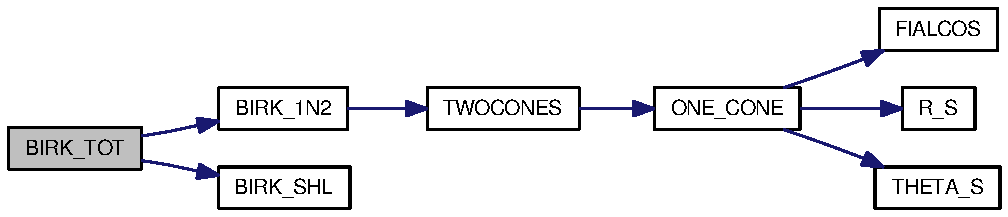
\includegraphics[width=260pt]{_tsyg2004_8c_a448f7ca5c043203dab6208c5c982571_cgraph}
\end{center}
\end{figure}


Here is the caller graph for this function:\nopagebreak
\begin{figure}[H]
\begin{center}
\leavevmode
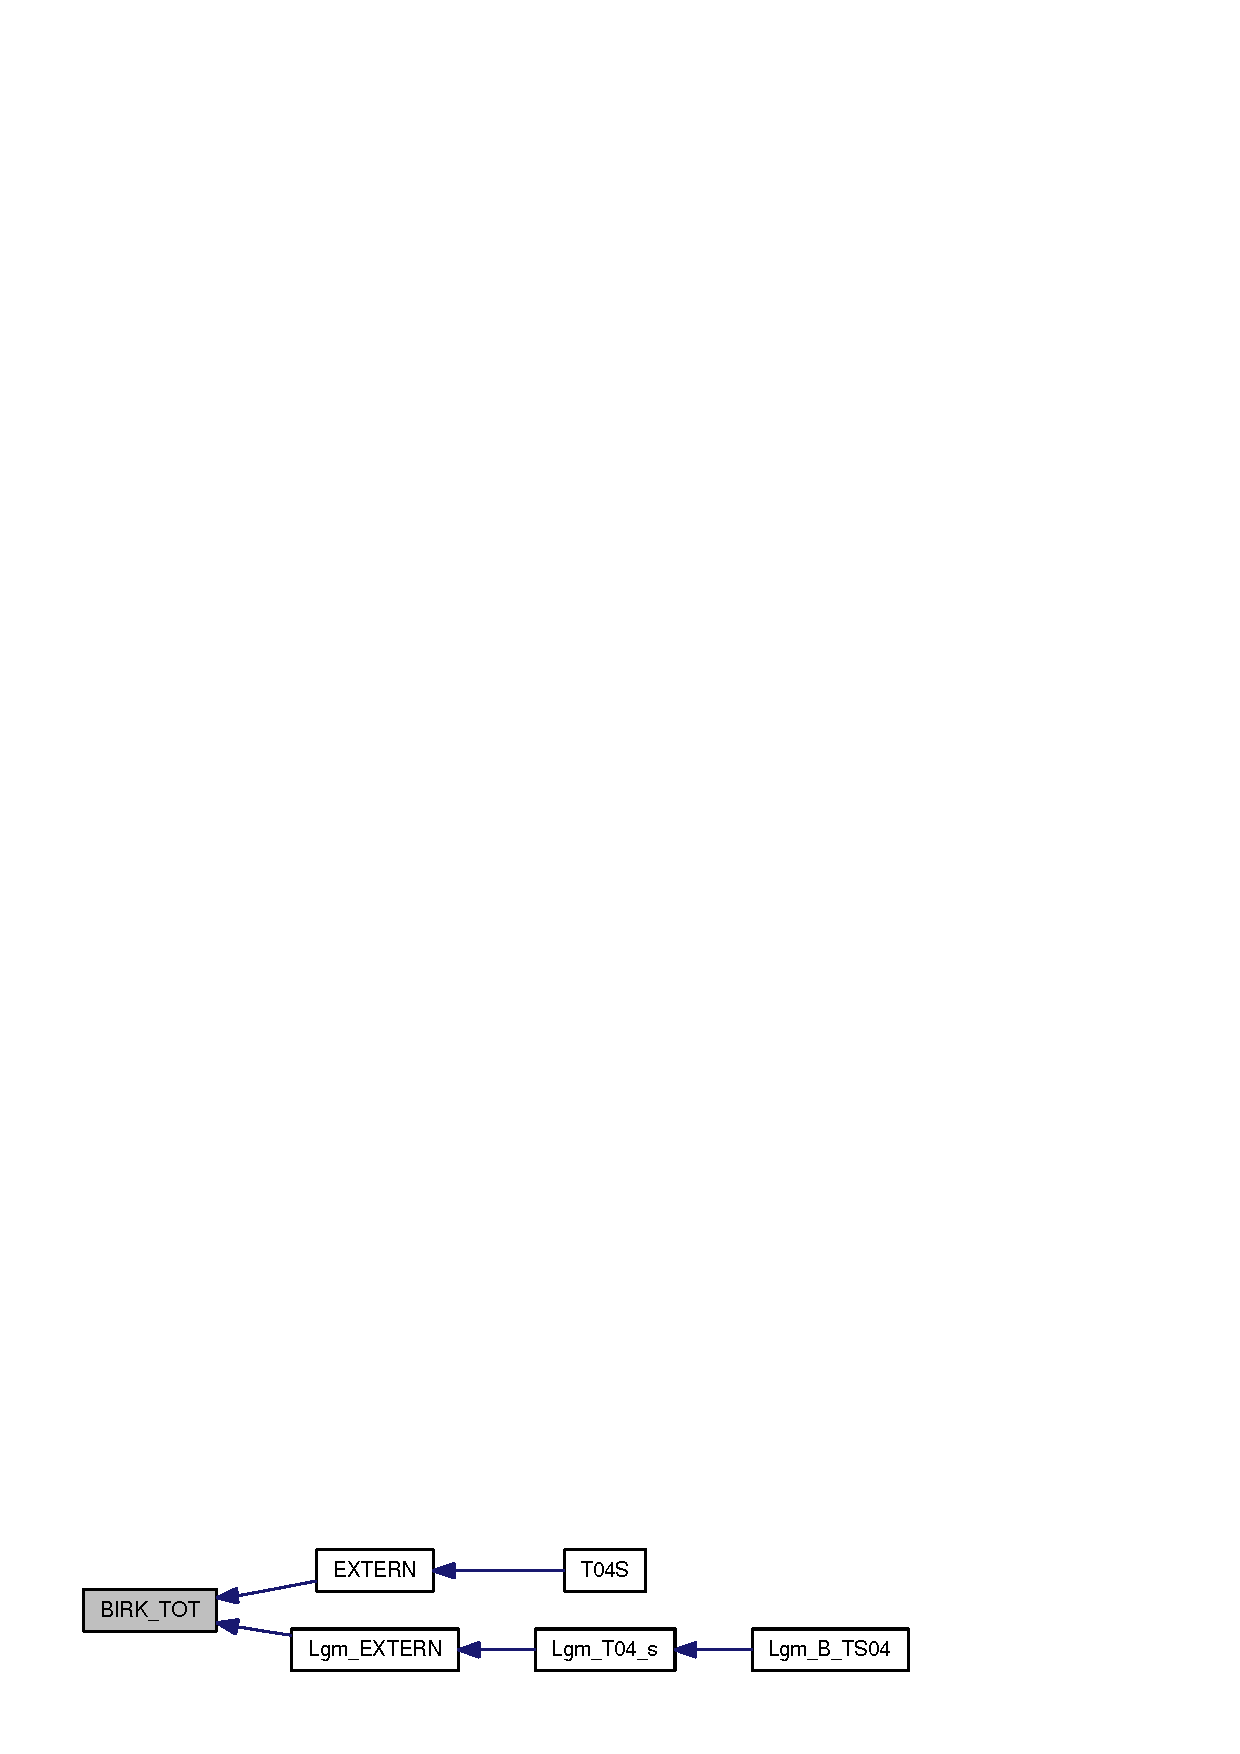
\includegraphics[width=220pt]{_tsyg2004_8c_a448f7ca5c043203dab6208c5c982571_icgraph}
\end{center}
\end{figure}
\hypertarget{_tsyg2004_8c_05b3a8c8d1e1b62725abe895df3d1ca1}{
\index{Tsyg2004.c@{Tsyg2004.c}!BIRK\_\-1N2@{BIRK\_\-1N2}}
\index{BIRK\_\-1N2@{BIRK\_\-1N2}!Tsyg2004.c@{Tsyg2004.c}}
\subsubsection[{BIRK\_\-1N2}]{\setlength{\rightskip}{0pt plus 5cm}void BIRK\_\-1N2 (int {\em NUMB}, \/  int {\em MODE}, \/  double {\em PS}, \/  double {\em X}, \/  double {\em Y}, \/  double {\em Z}, \/  double $\ast$ {\em BX}, \/  double $\ast$ {\em BY}, \/  double $\ast$ {\em BZ})}}
\label{_tsyg2004_8c_05b3a8c8d1e1b62725abe895df3d1ca1}




Definition at line 1469 of file Tsyg2004.c.

Here is the call graph for this function:\nopagebreak
\begin{figure}[H]
\begin{center}
\leavevmode
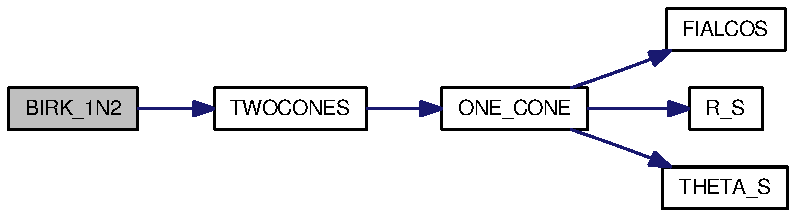
\includegraphics[width=209pt]{_tsyg2004_8c_05b3a8c8d1e1b62725abe895df3d1ca1_cgraph}
\end{center}
\end{figure}


Here is the caller graph for this function:\nopagebreak
\begin{figure}[H]
\begin{center}
\leavevmode
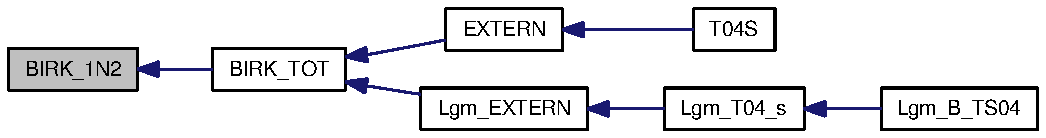
\includegraphics[width=269pt]{_tsyg2004_8c_05b3a8c8d1e1b62725abe895df3d1ca1_icgraph}
\end{center}
\end{figure}
\hypertarget{_tsyg2004_8c_b05c2844104041ea55de4c30aaa5b968}{
\index{Tsyg2004.c@{Tsyg2004.c}!TWOCONES@{TWOCONES}}
\index{TWOCONES@{TWOCONES}!Tsyg2004.c@{Tsyg2004.c}}
\subsubsection[{TWOCONES}]{\setlength{\rightskip}{0pt plus 5cm}void TWOCONES (double $\ast$ {\em A}, \/  double {\em X}, \/  double {\em Y}, \/  double {\em Z}, \/  double $\ast$ {\em BX}, \/  double $\ast$ {\em BY}, \/  double $\ast$ {\em BZ})}}
\label{_tsyg2004_8c_b05c2844104041ea55de4c30aaa5b968}




Definition at line 1605 of file Tsyg2004.c.

Here is the call graph for this function:\nopagebreak
\begin{figure}[H]
\begin{center}
\leavevmode
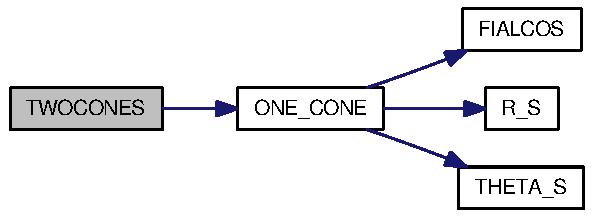
\includegraphics[width=160pt]{_tsyg2004_8c_b05c2844104041ea55de4c30aaa5b968_cgraph}
\end{center}
\end{figure}


Here is the caller graph for this function:\nopagebreak
\begin{figure}[H]
\begin{center}
\leavevmode
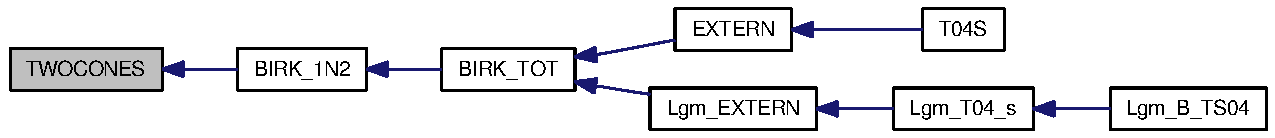
\includegraphics[width=324pt]{_tsyg2004_8c_b05c2844104041ea55de4c30aaa5b968_icgraph}
\end{center}
\end{figure}
\hypertarget{_tsyg2004_8c_d3ff91c1de1106c25ccbf3c1694cc883}{
\index{Tsyg2004.c@{Tsyg2004.c}!ONE\_\-CONE@{ONE\_\-CONE}}
\index{ONE\_\-CONE@{ONE\_\-CONE}!Tsyg2004.c@{Tsyg2004.c}}
\subsubsection[{ONE\_\-CONE}]{\setlength{\rightskip}{0pt plus 5cm}void ONE\_\-CONE (double $\ast$ {\em A}, \/  double {\em X}, \/  double {\em Y}, \/  double {\em Z}, \/  double $\ast$ {\em BX}, \/  double $\ast$ {\em BY}, \/  double $\ast$ {\em BZ})}}
\label{_tsyg2004_8c_d3ff91c1de1106c25ccbf3c1694cc883}




Definition at line 1627 of file Tsyg2004.c.

Here is the call graph for this function:\nopagebreak
\begin{figure}[H]
\begin{center}
\leavevmode
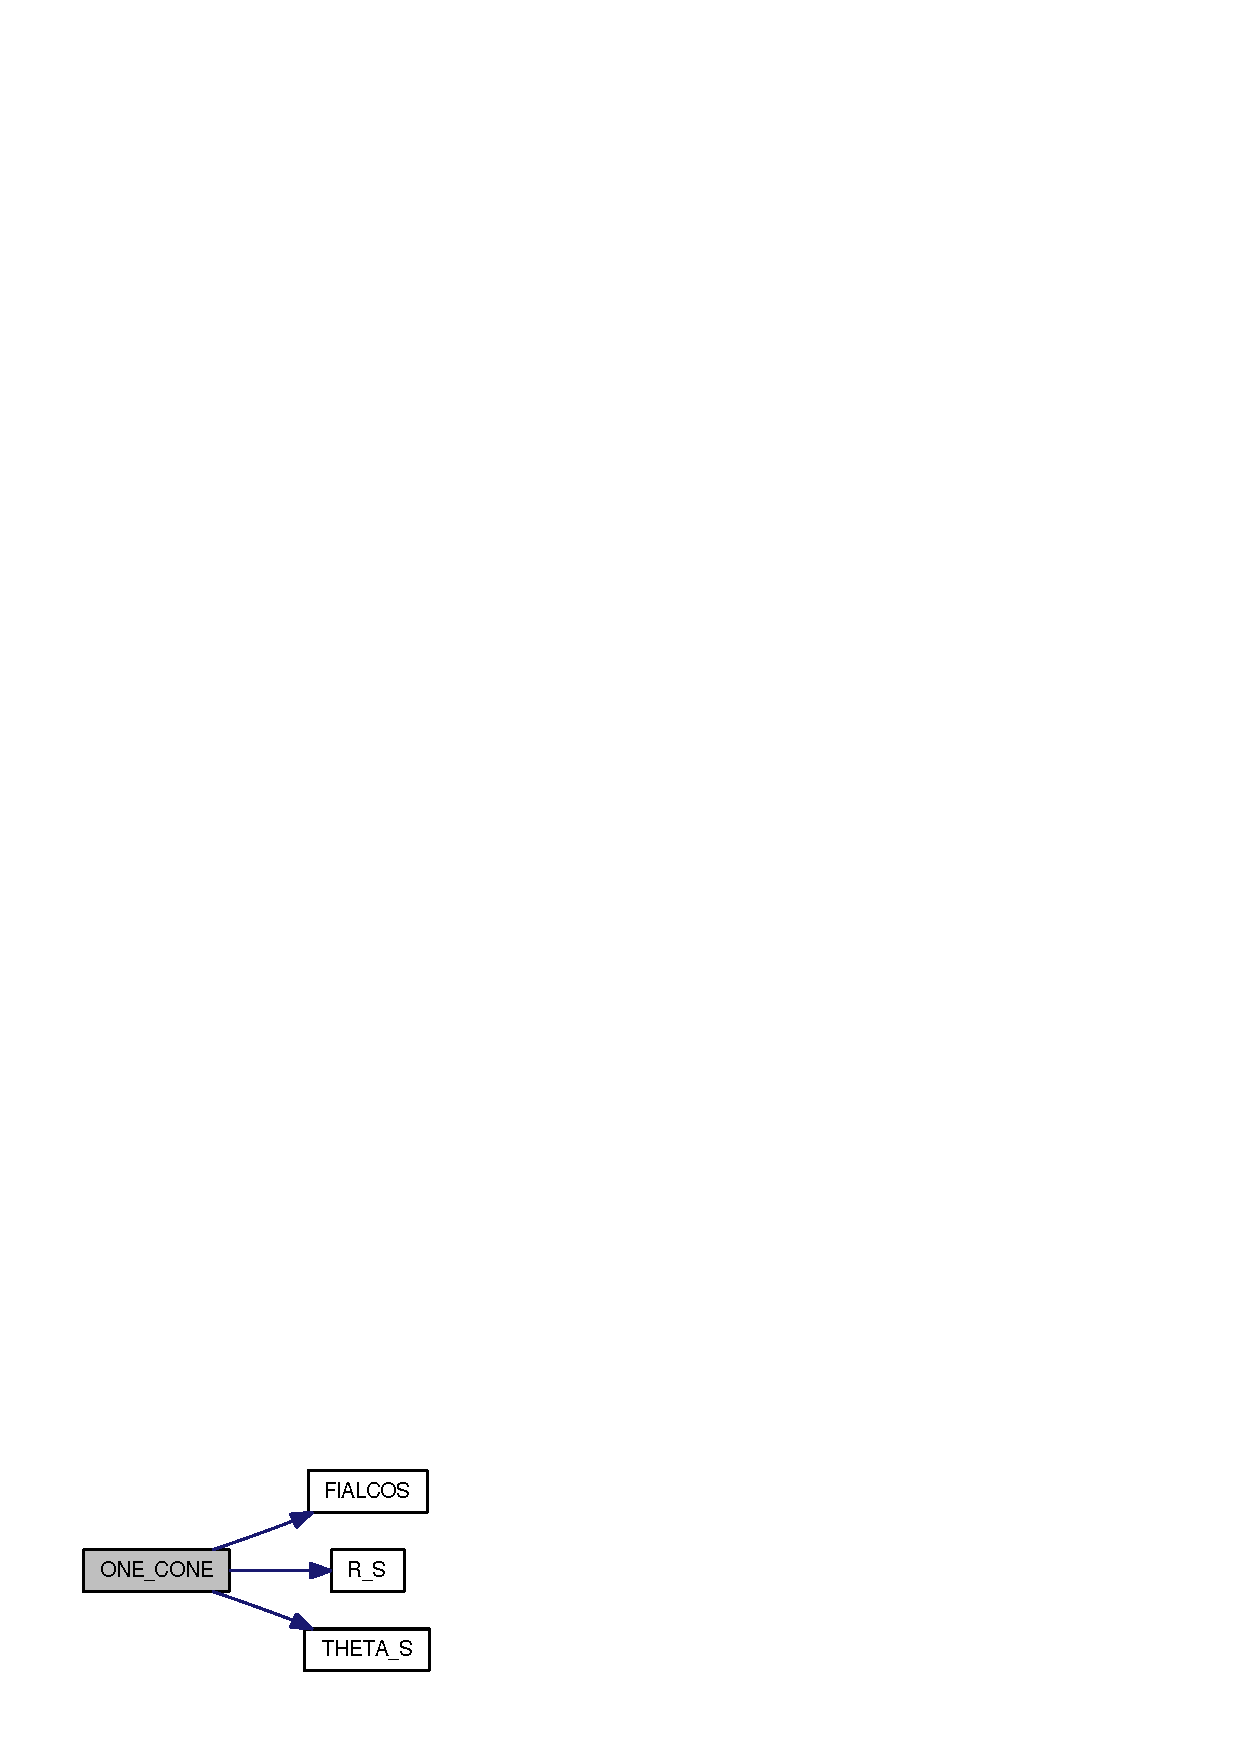
\includegraphics[width=105pt]{_tsyg2004_8c_d3ff91c1de1106c25ccbf3c1694cc883_cgraph}
\end{center}
\end{figure}


Here is the caller graph for this function:\nopagebreak
\begin{figure}[H]
\begin{center}
\leavevmode
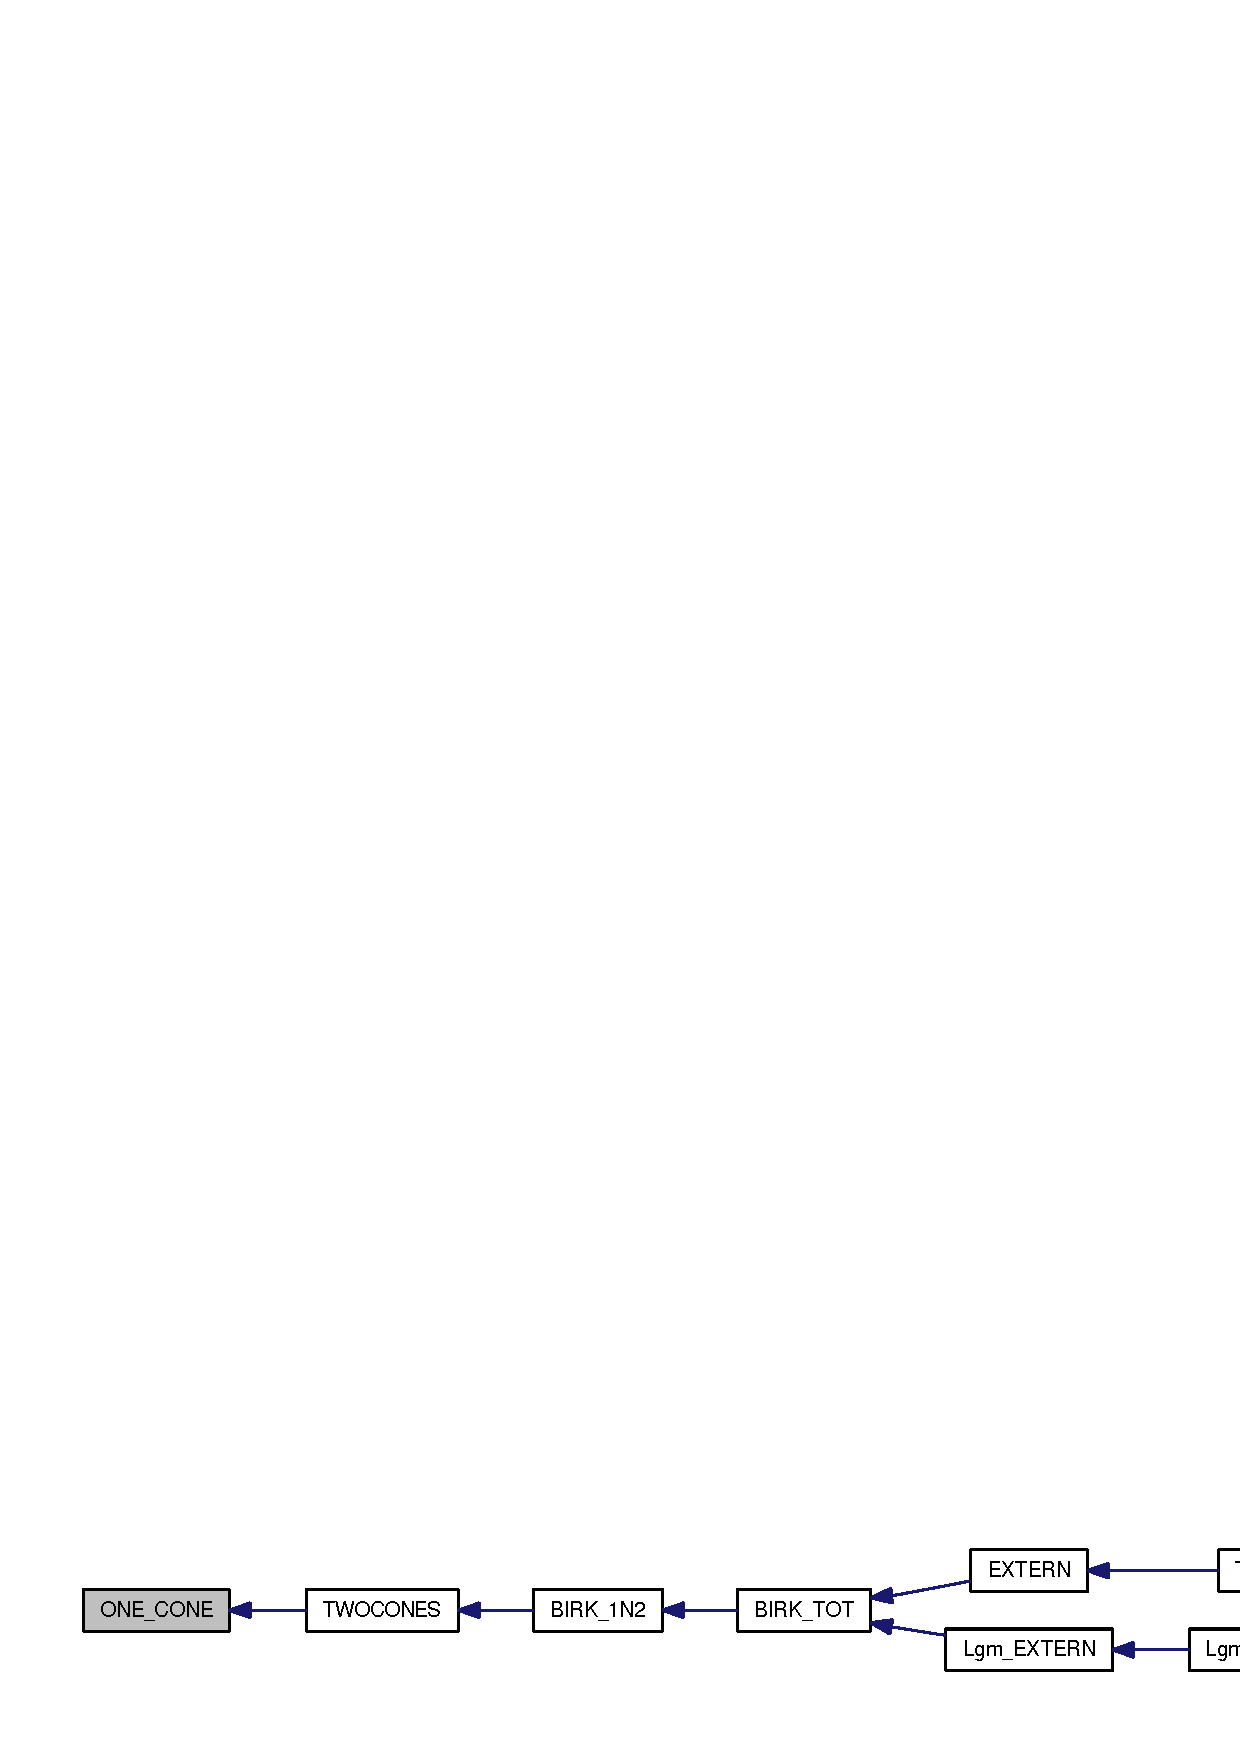
\includegraphics[width=377pt]{_tsyg2004_8c_d3ff91c1de1106c25ccbf3c1694cc883_icgraph}
\end{center}
\end{figure}
\hypertarget{_tsyg2004_8c_af80d04276fc0dce8abc24392512cf8e}{
\index{Tsyg2004.c@{Tsyg2004.c}!THETA\_\-S@{THETA\_\-S}}
\index{THETA\_\-S@{THETA\_\-S}!Tsyg2004.c@{Tsyg2004.c}}
\subsubsection[{THETA\_\-S}]{\setlength{\rightskip}{0pt plus 5cm}double THETA\_\-S (double $\ast$ {\em A}, \/  double {\em R}, \/  double {\em THETA})}}
\label{_tsyg2004_8c_af80d04276fc0dce8abc24392512cf8e}




Definition at line 1721 of file Tsyg2004.c.

Here is the caller graph for this function:\nopagebreak
\begin{figure}[H]
\begin{center}
\leavevmode
\includegraphics[width=420pt]{_tsyg2004_8c_af80d04276fc0dce8abc24392512cf8e_icgraph}
\end{center}
\end{figure}
\hypertarget{_tsyg2004_8c_22701b7ad2e702887750fdec469f01fb}{
\index{Tsyg2004.c@{Tsyg2004.c}!R\_\-S@{R\_\-S}}
\index{R\_\-S@{R\_\-S}!Tsyg2004.c@{Tsyg2004.c}}
\subsubsection[{R\_\-S}]{\setlength{\rightskip}{0pt plus 5cm}double R\_\-S (double $\ast$ {\em A}, \/  double {\em R}, \/  double {\em THETA})}}
\label{_tsyg2004_8c_22701b7ad2e702887750fdec469f01fb}




Definition at line 1701 of file Tsyg2004.c.

Here is the caller graph for this function:\nopagebreak
\begin{figure}[H]
\begin{center}
\leavevmode
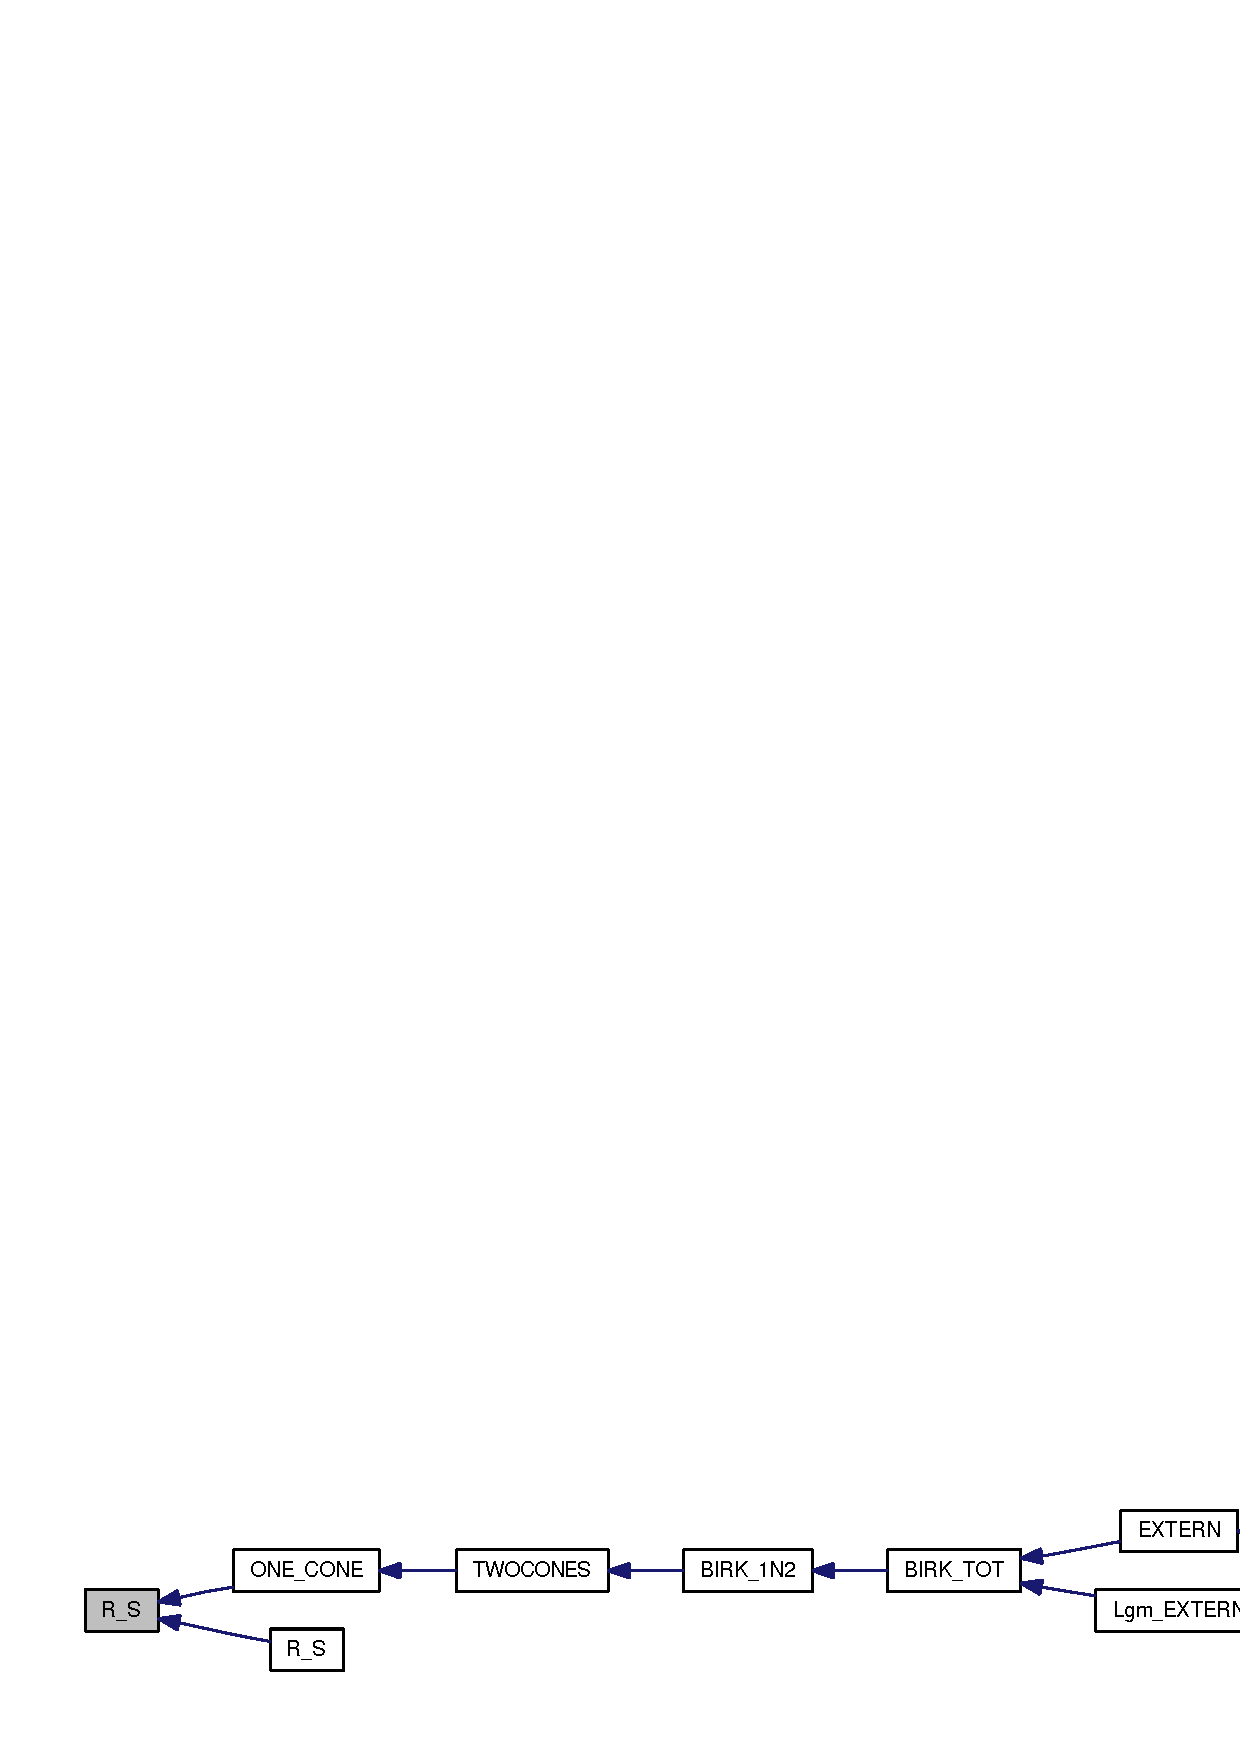
\includegraphics[width=413pt]{_tsyg2004_8c_22701b7ad2e702887750fdec469f01fb_icgraph}
\end{center}
\end{figure}
\hypertarget{_tsyg2004_8c_8e93acc99263e229c4b81a6c4cd9f148}{
\index{Tsyg2004.c@{Tsyg2004.c}!FIALCOS@{FIALCOS}}
\index{FIALCOS@{FIALCOS}!Tsyg2004.c@{Tsyg2004.c}}
\subsubsection[{FIALCOS}]{\setlength{\rightskip}{0pt plus 5cm}void FIALCOS (double {\em R}, \/  double {\em THETA}, \/  double {\em PHI}, \/  double $\ast$ {\em BTHETA}, \/  double $\ast$ {\em BPHI}, \/  int {\em N}, \/  double {\em THETA0}, \/  double {\em DT})}}
\label{_tsyg2004_8c_8e93acc99263e229c4b81a6c4cd9f148}




Definition at line 1742 of file Tsyg2004.c.

Here is the caller graph for this function:\nopagebreak
\begin{figure}[H]
\begin{center}
\leavevmode
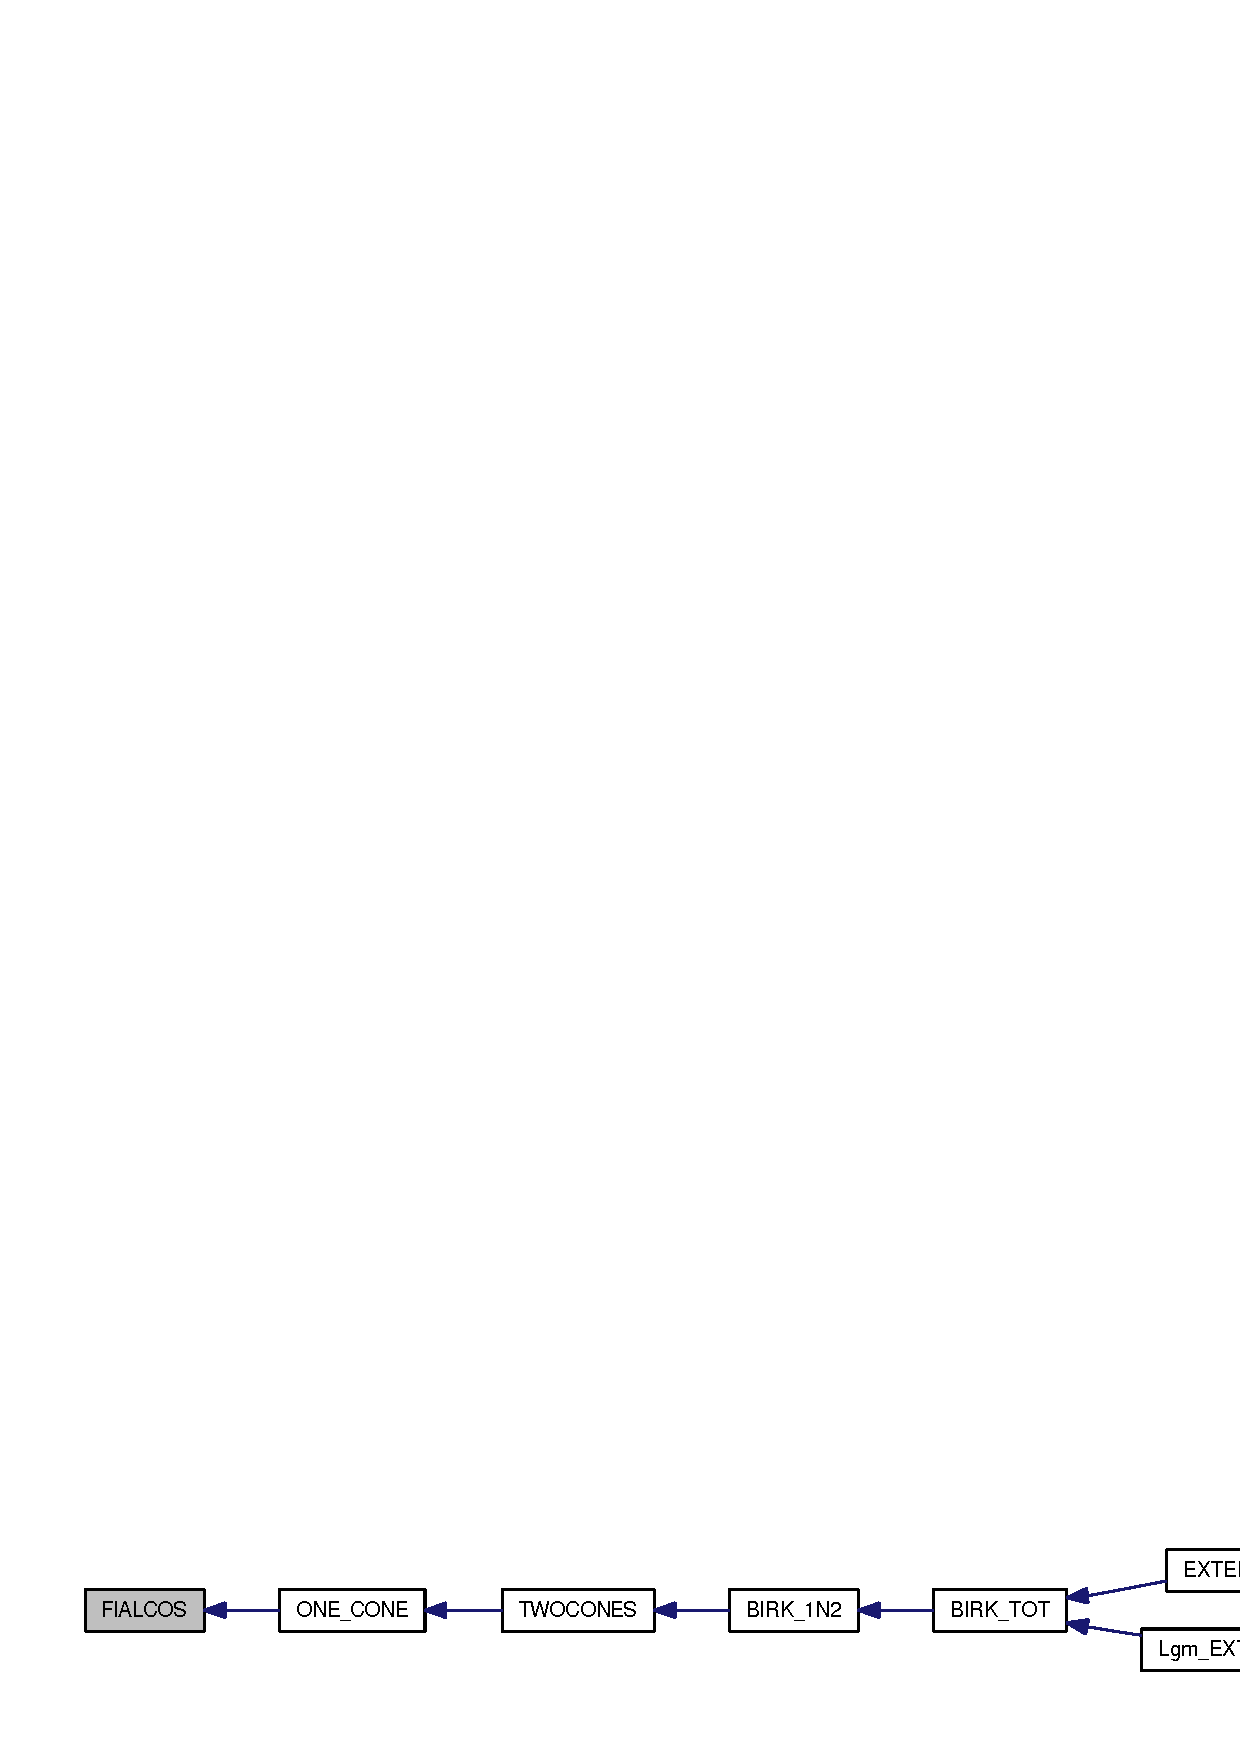
\includegraphics[width=420pt]{_tsyg2004_8c_8e93acc99263e229c4b81a6c4cd9f148_icgraph}
\end{center}
\end{figure}
\hypertarget{_tsyg2004_8c_723d4ced4ac10c32344d63bda6126fdf}{
\index{Tsyg2004.c@{Tsyg2004.c}!BIRK\_\-SHL@{BIRK\_\-SHL}}
\index{BIRK\_\-SHL@{BIRK\_\-SHL}!Tsyg2004.c@{Tsyg2004.c}}
\subsubsection[{BIRK\_\-SHL}]{\setlength{\rightskip}{0pt plus 5cm}void BIRK\_\-SHL (int {\em J}, \/  int {\em PSChanged}, \/  int {\em XChanged}, \/  int {\em YChanged}, \/  int {\em ZChanged}, \/  double $\ast$ {\em A}, \/  double {\em PS}, \/  double {\em X\_\-SC}, \/  double {\em X}, \/  double {\em Y}, \/  double {\em Z}, \/  double $\ast$ {\em BX}, \/  double $\ast$ {\em BY}, \/  double $\ast$ {\em BZ})}}
\label{_tsyg2004_8c_723d4ced4ac10c32344d63bda6126fdf}




Definition at line 1828 of file Tsyg2004.c.

Here is the caller graph for this function:\nopagebreak
\begin{figure}[H]
\begin{center}
\leavevmode
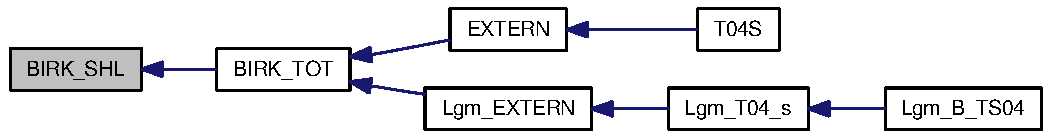
\includegraphics[width=270pt]{_tsyg2004_8c_723d4ced4ac10c32344d63bda6126fdf_icgraph}
\end{center}
\end{figure}
\hypertarget{_tsyg2004_8c_2a492ba836369d99dfb597c1675f6a33}{
\index{Tsyg2004.c@{Tsyg2004.c}!FULL\_\-RC@{FULL\_\-RC}}
\index{FULL\_\-RC@{FULL\_\-RC}!Tsyg2004.c@{Tsyg2004.c}}
\subsubsection[{FULL\_\-RC}]{\setlength{\rightskip}{0pt plus 5cm}void FULL\_\-RC (int {\em IOPR}, \/  double {\em PS}, \/  double {\em X}, \/  double {\em Y}, \/  double {\em Z}, \/  double $\ast$ {\em BXSRC}, \/  double $\ast$ {\em BYSRC}, \/  double $\ast$ {\em BZSRC}, \/  double $\ast$ {\em BXPRC}, \/  double $\ast$ {\em BYPRC}, \/  double $\ast$ {\em BZPRC})}}
\label{_tsyg2004_8c_2a492ba836369d99dfb597c1675f6a33}




Definition at line 2051 of file Tsyg2004.c.

Here is the call graph for this function:\nopagebreak
\begin{figure}[H]
\begin{center}
\leavevmode
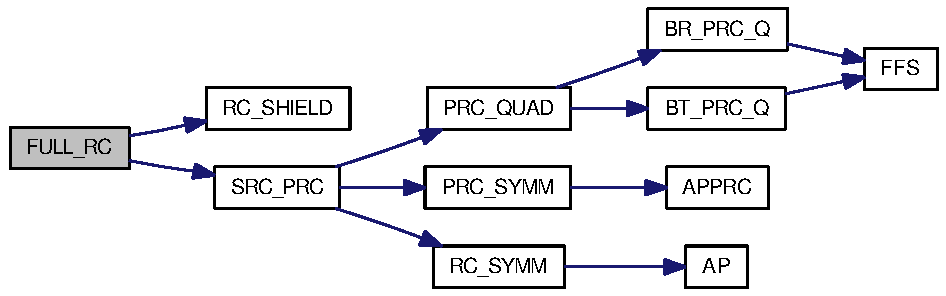
\includegraphics[width=245pt]{_tsyg2004_8c_2a492ba836369d99dfb597c1675f6a33_cgraph}
\end{center}
\end{figure}


Here is the caller graph for this function:\nopagebreak
\begin{figure}[H]
\begin{center}
\leavevmode
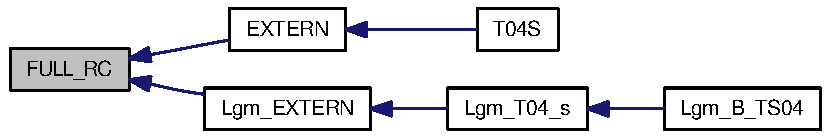
\includegraphics[width=217pt]{_tsyg2004_8c_2a492ba836369d99dfb597c1675f6a33_icgraph}
\end{center}
\end{figure}
\hypertarget{_tsyg2004_8c_9d8e16b4209da2c6896cb9fb1531f2fa}{
\index{Tsyg2004.c@{Tsyg2004.c}!SRC\_\-PRC@{SRC\_\-PRC}}
\index{SRC\_\-PRC@{SRC\_\-PRC}!Tsyg2004.c@{Tsyg2004.c}}
\subsubsection[{SRC\_\-PRC}]{\setlength{\rightskip}{0pt plus 5cm}void SRC\_\-PRC (int {\em IOPR}, \/  double {\em SC\_\-SY}, \/  double {\em SC\_\-PR}, \/  double {\em PHI}, \/  double {\em PS}, \/  double {\em X}, \/  double {\em Y}, \/  double {\em Z}, \/  double $\ast$ {\em BXSRC}, \/  double $\ast$ {\em BYSRC}, \/  double $\ast$ {\em BZSRC}, \/  double $\ast$ {\em BXPRC}, \/  double $\ast$ {\em BYPRC}, \/  double $\ast$ {\em BZPRC})}}
\label{_tsyg2004_8c_9d8e16b4209da2c6896cb9fb1531f2fa}




Definition at line 2146 of file Tsyg2004.c.

Here is the call graph for this function:\nopagebreak
\begin{figure}[H]
\begin{center}
\leavevmode
\includegraphics[width=193pt]{_tsyg2004_8c_9d8e16b4209da2c6896cb9fb1531f2fa_cgraph}
\end{center}
\end{figure}


Here is the caller graph for this function:\nopagebreak
\begin{figure}[H]
\begin{center}
\leavevmode
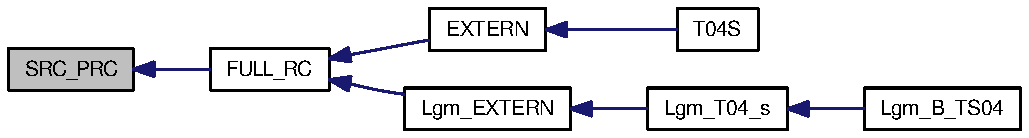
\includegraphics[width=265pt]{_tsyg2004_8c_9d8e16b4209da2c6896cb9fb1531f2fa_icgraph}
\end{center}
\end{figure}
\hypertarget{_tsyg2004_8c_16ec50640c104c5c2a57ef6a51b21f01}{
\index{Tsyg2004.c@{Tsyg2004.c}!RC\_\-SYMM@{RC\_\-SYMM}}
\index{RC\_\-SYMM@{RC\_\-SYMM}!Tsyg2004.c@{Tsyg2004.c}}
\subsubsection[{RC\_\-SYMM}]{\setlength{\rightskip}{0pt plus 5cm}void RC\_\-SYMM (double {\em X}, \/  double {\em Y}, \/  double {\em Z}, \/  double $\ast$ {\em BX}, \/  double $\ast$ {\em BY}, \/  double $\ast$ {\em BZ})}}
\label{_tsyg2004_8c_16ec50640c104c5c2a57ef6a51b21f01}




Definition at line 2242 of file Tsyg2004.c.

Here is the call graph for this function:\nopagebreak
\begin{figure}[H]
\begin{center}
\leavevmode
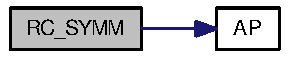
\includegraphics[width=87pt]{_tsyg2004_8c_16ec50640c104c5c2a57ef6a51b21f01_cgraph}
\end{center}
\end{figure}


Here is the caller graph for this function:\nopagebreak
\begin{figure}[H]
\begin{center}
\leavevmode
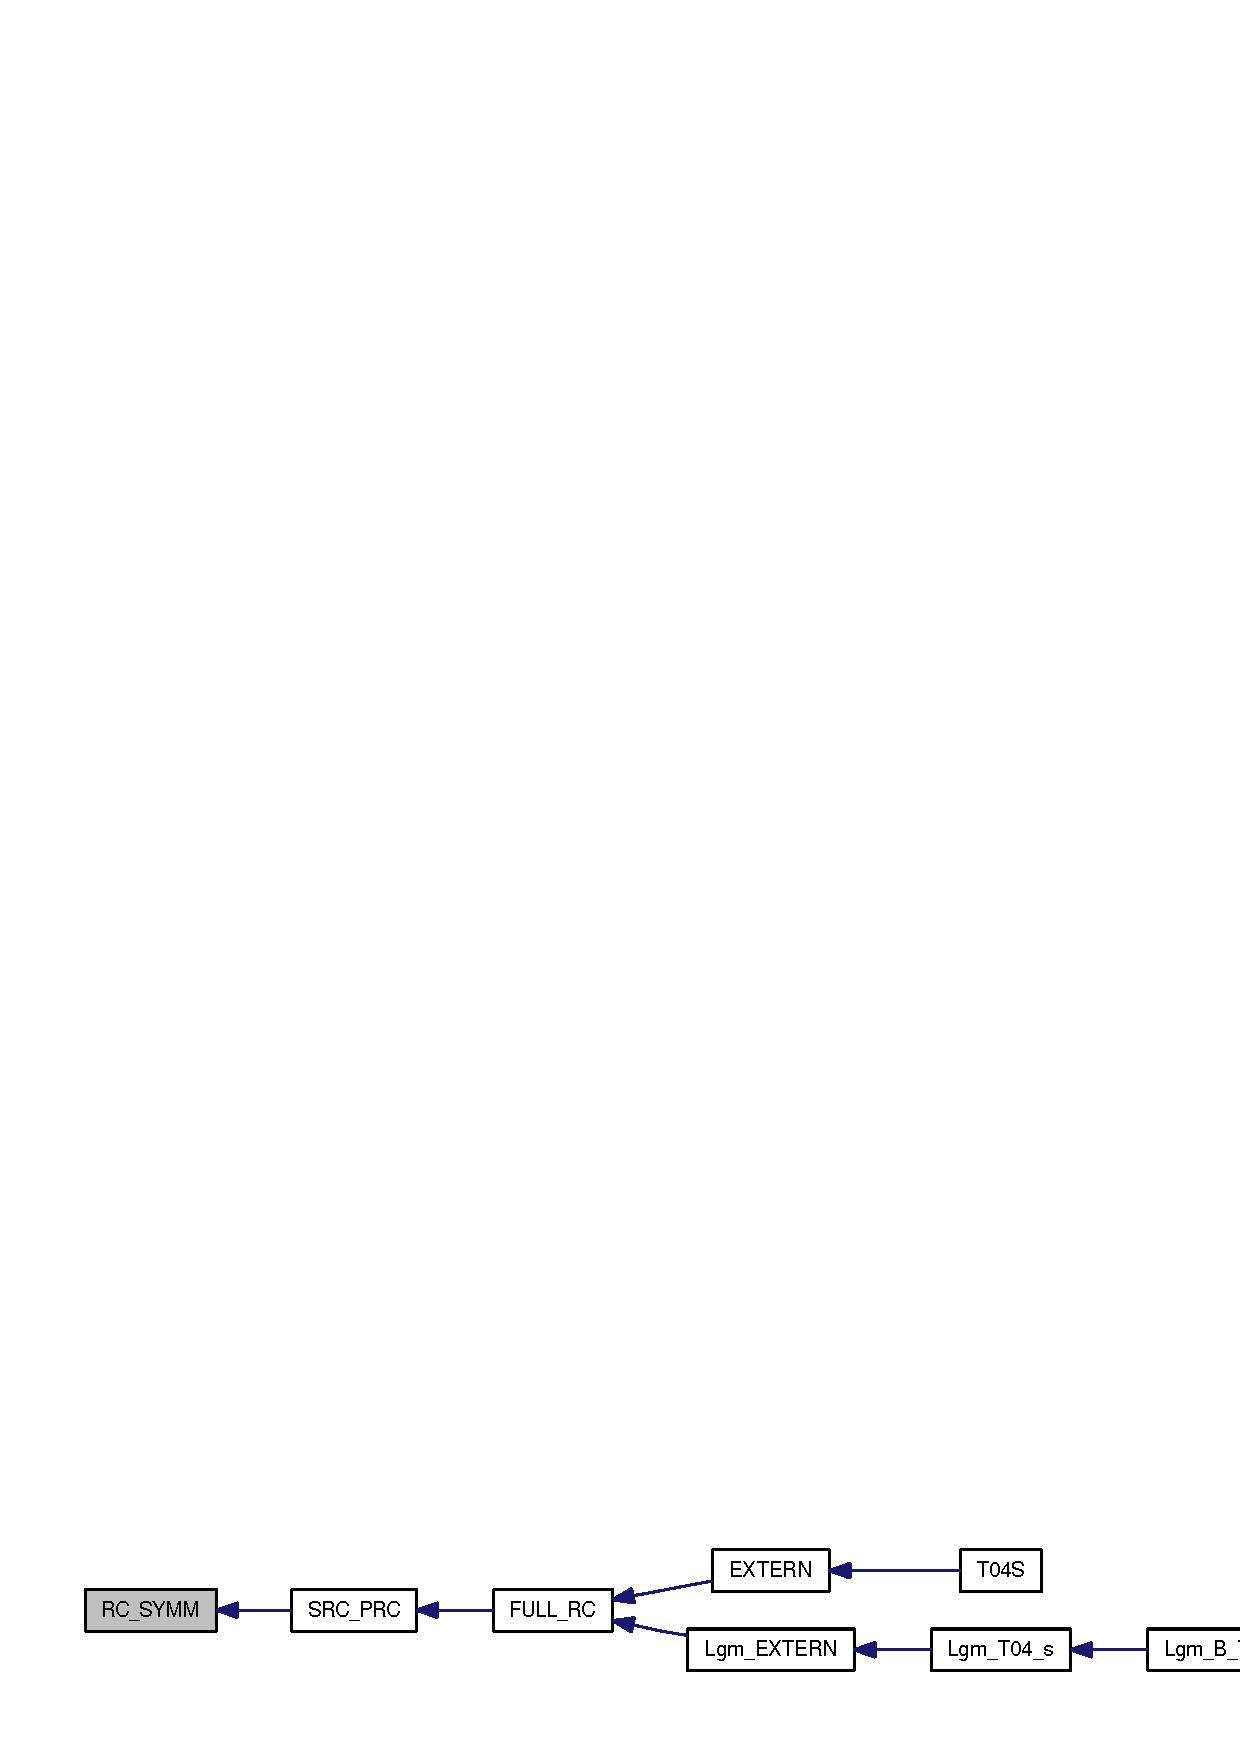
\includegraphics[width=315pt]{_tsyg2004_8c_16ec50640c104c5c2a57ef6a51b21f01_icgraph}
\end{center}
\end{figure}
\hypertarget{_tsyg2004_8c_55f2b5b45100a3e191f3423e007d7174}{
\index{Tsyg2004.c@{Tsyg2004.c}!AP@{AP}}
\index{AP@{AP}!Tsyg2004.c@{Tsyg2004.c}}
\subsubsection[{AP}]{\setlength{\rightskip}{0pt plus 5cm}double AP (double {\em R}, \/  double {\em SINT}, \/  double {\em COST})}}
\label{_tsyg2004_8c_55f2b5b45100a3e191f3423e007d7174}




Definition at line 2292 of file Tsyg2004.c.

Here is the caller graph for this function:\nopagebreak
\begin{figure}[H]
\begin{center}
\leavevmode
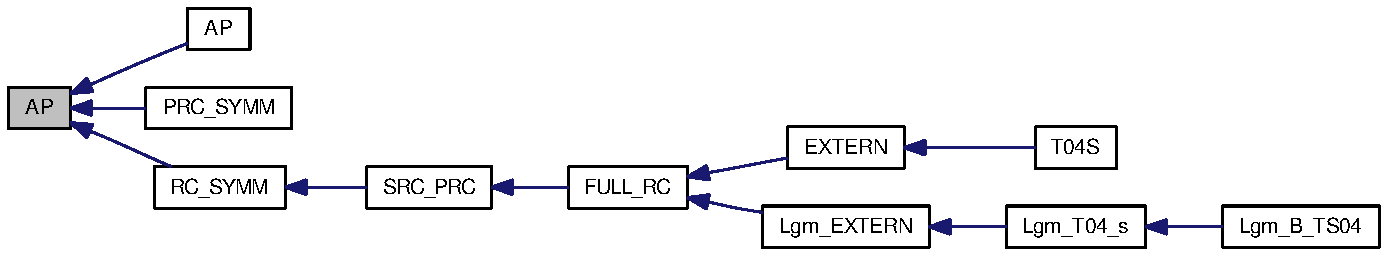
\includegraphics[width=351pt]{_tsyg2004_8c_55f2b5b45100a3e191f3423e007d7174_icgraph}
\end{center}
\end{figure}
\hypertarget{_tsyg2004_8c_a49661b45ed199138df07d1806ad7240}{
\index{Tsyg2004.c@{Tsyg2004.c}!PRC\_\-SYMM@{PRC\_\-SYMM}}
\index{PRC\_\-SYMM@{PRC\_\-SYMM}!Tsyg2004.c@{Tsyg2004.c}}
\subsubsection[{PRC\_\-SYMM}]{\setlength{\rightskip}{0pt plus 5cm}void PRC\_\-SYMM (double {\em X}, \/  double {\em Y}, \/  double {\em Z}, \/  double $\ast$ {\em BX}, \/  double $\ast$ {\em BY}, \/  double $\ast$ {\em BZ})}}
\label{_tsyg2004_8c_a49661b45ed199138df07d1806ad7240}




Definition at line 2428 of file Tsyg2004.c.

Here is the call graph for this function:\nopagebreak
\begin{figure}[H]
\begin{center}
\leavevmode
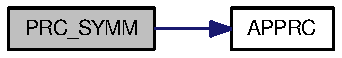
\includegraphics[width=100pt]{_tsyg2004_8c_a49661b45ed199138df07d1806ad7240_cgraph}
\end{center}
\end{figure}


Here is the caller graph for this function:\nopagebreak
\begin{figure}[H]
\begin{center}
\leavevmode
\includegraphics[width=318pt]{_tsyg2004_8c_a49661b45ed199138df07d1806ad7240_icgraph}
\end{center}
\end{figure}
\hypertarget{_tsyg2004_8c_184ae8e5e4f65974829d3ff56683be12}{
\index{Tsyg2004.c@{Tsyg2004.c}!APPRC@{APPRC}}
\index{APPRC@{APPRC}!Tsyg2004.c@{Tsyg2004.c}}
\subsubsection[{APPRC}]{\setlength{\rightskip}{0pt plus 5cm}double APPRC (double {\em R}, \/  double {\em SINT}, \/  double {\em COST})}}
\label{_tsyg2004_8c_184ae8e5e4f65974829d3ff56683be12}




Definition at line 2476 of file Tsyg2004.c.

Here is the caller graph for this function:\nopagebreak
\begin{figure}[H]
\begin{center}
\leavevmode
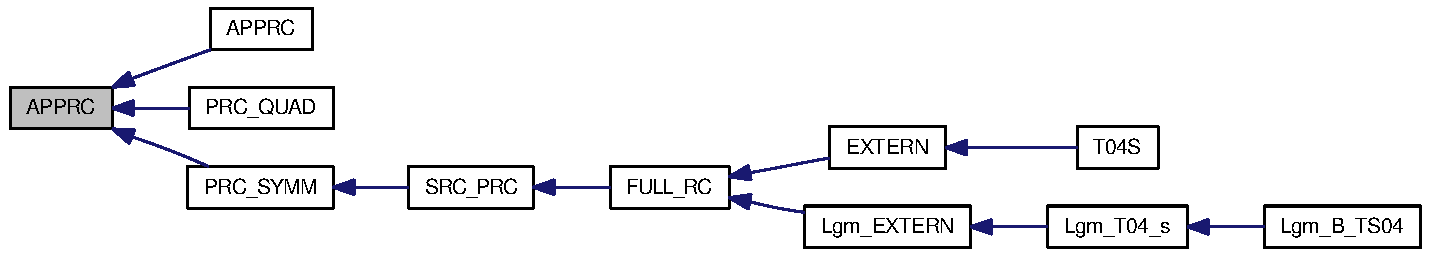
\includegraphics[width=361pt]{_tsyg2004_8c_184ae8e5e4f65974829d3ff56683be12_icgraph}
\end{center}
\end{figure}
\hypertarget{_tsyg2004_8c_7d3132f7a6ed31b467740063133da1fe}{
\index{Tsyg2004.c@{Tsyg2004.c}!PRC\_\-QUAD@{PRC\_\-QUAD}}
\index{PRC\_\-QUAD@{PRC\_\-QUAD}!Tsyg2004.c@{Tsyg2004.c}}
\subsubsection[{PRC\_\-QUAD}]{\setlength{\rightskip}{0pt plus 5cm}void PRC\_\-QUAD (double {\em X}, \/  double {\em Y}, \/  double {\em Z}, \/  double $\ast$ {\em BX}, \/  double $\ast$ {\em BY}, \/  double $\ast$ {\em BZ})}}
\label{_tsyg2004_8c_7d3132f7a6ed31b467740063133da1fe}




Definition at line 2628 of file Tsyg2004.c.

Here is the call graph for this function:\nopagebreak
\begin{figure}[H]
\begin{center}
\leavevmode
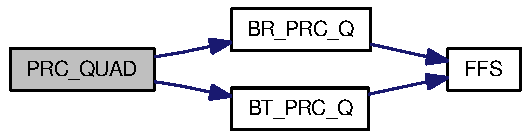
\includegraphics[width=145pt]{_tsyg2004_8c_7d3132f7a6ed31b467740063133da1fe_cgraph}
\end{center}
\end{figure}


Here is the caller graph for this function:\nopagebreak
\begin{figure}[H]
\begin{center}
\leavevmode
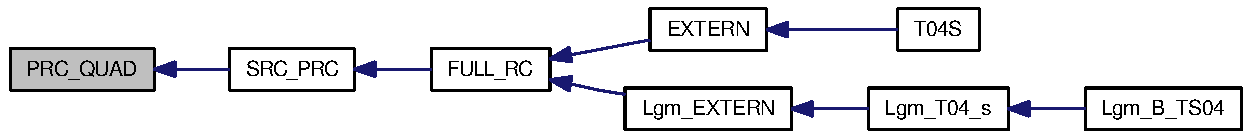
\includegraphics[width=318pt]{_tsyg2004_8c_7d3132f7a6ed31b467740063133da1fe_icgraph}
\end{center}
\end{figure}
\hypertarget{_tsyg2004_8c_51ea88e5a0772dd9763092b23868d83e}{
\index{Tsyg2004.c@{Tsyg2004.c}!BR\_\-PRC\_\-Q@{BR\_\-PRC\_\-Q}}
\index{BR\_\-PRC\_\-Q@{BR\_\-PRC\_\-Q}!Tsyg2004.c@{Tsyg2004.c}}
\subsubsection[{BR\_\-PRC\_\-Q}]{\setlength{\rightskip}{0pt plus 5cm}double BR\_\-PRC\_\-Q (double {\em R}, \/  double {\em SINT}, \/  double {\em COST})}}
\label{_tsyg2004_8c_51ea88e5a0772dd9763092b23868d83e}




Definition at line 2693 of file Tsyg2004.c.

Here is the call graph for this function:\nopagebreak
\begin{figure}[H]
\begin{center}
\leavevmode
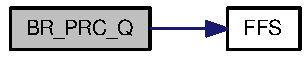
\includegraphics[width=92pt]{_tsyg2004_8c_51ea88e5a0772dd9763092b23868d83e_cgraph}
\end{center}
\end{figure}


Here is the caller graph for this function:\nopagebreak
\begin{figure}[H]
\begin{center}
\leavevmode
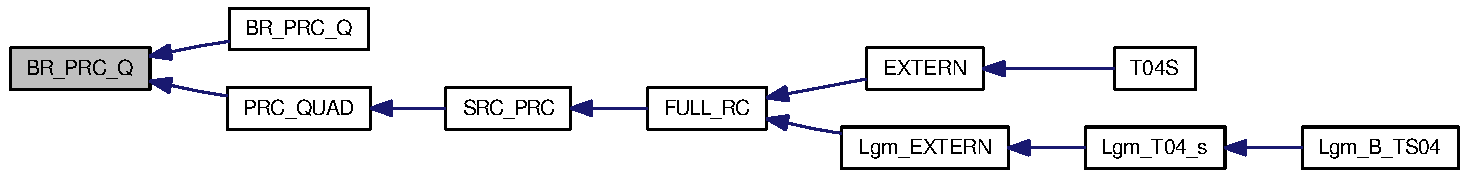
\includegraphics[width=370pt]{_tsyg2004_8c_51ea88e5a0772dd9763092b23868d83e_icgraph}
\end{center}
\end{figure}
\hypertarget{_tsyg2004_8c_40293e54c4b1290d9463ec556292303b}{
\index{Tsyg2004.c@{Tsyg2004.c}!BT\_\-PRC\_\-Q@{BT\_\-PRC\_\-Q}}
\index{BT\_\-PRC\_\-Q@{BT\_\-PRC\_\-Q}!Tsyg2004.c@{Tsyg2004.c}}
\subsubsection[{BT\_\-PRC\_\-Q}]{\setlength{\rightskip}{0pt plus 5cm}double BT\_\-PRC\_\-Q (double {\em R}, \/  double {\em SINT}, \/  double {\em COST})}}
\label{_tsyg2004_8c_40293e54c4b1290d9463ec556292303b}




Definition at line 2780 of file Tsyg2004.c.

Here is the call graph for this function:\nopagebreak
\begin{figure}[H]
\begin{center}
\leavevmode
\includegraphics[width=91pt]{_tsyg2004_8c_40293e54c4b1290d9463ec556292303b_cgraph}
\end{center}
\end{figure}


Here is the caller graph for this function:\nopagebreak
\begin{figure}[H]
\begin{center}
\leavevmode
\includegraphics[width=369pt]{_tsyg2004_8c_40293e54c4b1290d9463ec556292303b_icgraph}
\end{center}
\end{figure}
\hypertarget{_tsyg2004_8c_e9137c27c3c66aef974f6c4017b6ab9d}{
\index{Tsyg2004.c@{Tsyg2004.c}!FFS@{FFS}}
\index{FFS@{FFS}!Tsyg2004.c@{Tsyg2004.c}}
\subsubsection[{FFS}]{\setlength{\rightskip}{0pt plus 5cm}void FFS (double {\em A}, \/  double {\em A0}, \/  double {\em DA}, \/  double $\ast$ {\em F}, \/  double $\ast$ {\em FA}, \/  double $\ast$ {\em FS})}}
\label{_tsyg2004_8c_e9137c27c3c66aef974f6c4017b6ab9d}




Definition at line 2856 of file Tsyg2004.c.

Here is the caller graph for this function:\nopagebreak
\begin{figure}[H]
\begin{center}
\leavevmode
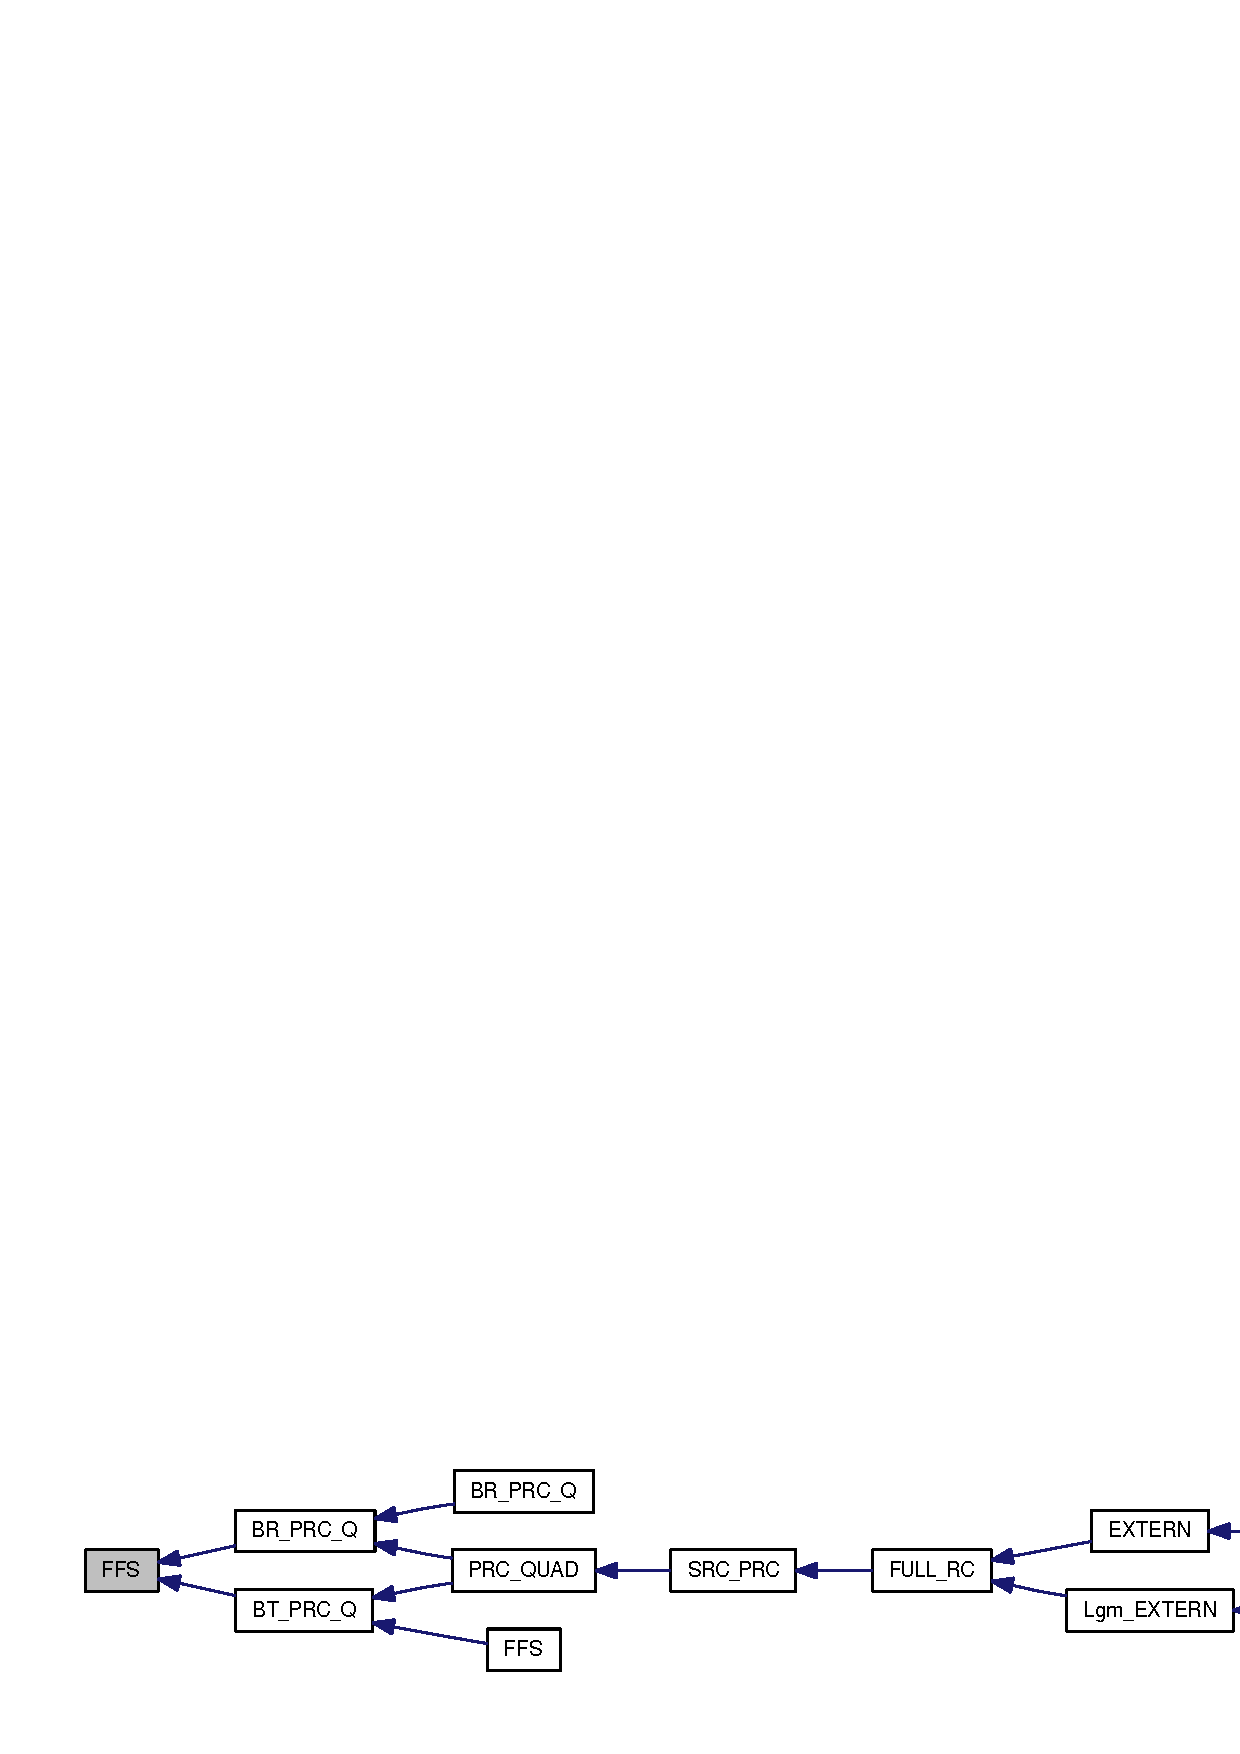
\includegraphics[width=406pt]{_tsyg2004_8c_e9137c27c3c66aef974f6c4017b6ab9d_icgraph}
\end{center}
\end{figure}
\hypertarget{_tsyg2004_8c_ae1fabae2232fcfa073907bc921dbf66}{
\index{Tsyg2004.c@{Tsyg2004.c}!RC\_\-SHIELD@{RC\_\-SHIELD}}
\index{RC\_\-SHIELD@{RC\_\-SHIELD}!Tsyg2004.c@{Tsyg2004.c}}
\subsubsection[{RC\_\-SHIELD}]{\setlength{\rightskip}{0pt plus 5cm}void RC\_\-SHIELD (double $\ast$ {\em A}, \/  double {\em PS}, \/  double {\em X\_\-SC}, \/  double {\em X}, \/  double {\em Y}, \/  double {\em Z}, \/  double $\ast$ {\em BX}, \/  double $\ast$ {\em BY}, \/  double $\ast$ {\em BZ})}}
\label{_tsyg2004_8c_ae1fabae2232fcfa073907bc921dbf66}




Definition at line 2876 of file Tsyg2004.c.

Here is the caller graph for this function:\nopagebreak
\begin{figure}[H]
\begin{center}
\leavevmode
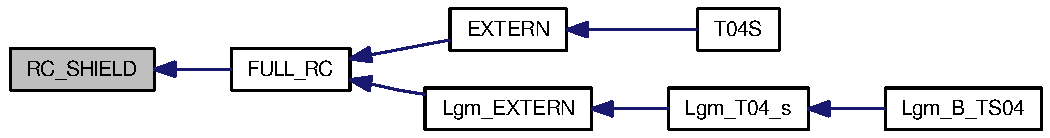
\includegraphics[width=270pt]{_tsyg2004_8c_ae1fabae2232fcfa073907bc921dbf66_icgraph}
\end{center}
\end{figure}
\hypertarget{_tsyg2004_8c_b1ff14f59abcc09994d8743db9a8f736}{
\index{Tsyg2004.c@{Tsyg2004.c}!DIPOLE@{DIPOLE}}
\index{DIPOLE@{DIPOLE}!Tsyg2004.c@{Tsyg2004.c}}
\subsubsection[{DIPOLE}]{\setlength{\rightskip}{0pt plus 5cm}void DIPOLE (double {\em PS}, \/  double {\em X}, \/  double {\em Y}, \/  double {\em Z}, \/  double $\ast$ {\em BX}, \/  double $\ast$ {\em BY}, \/  double $\ast$ {\em BZ})}}
\label{_tsyg2004_8c_b1ff14f59abcc09994d8743db9a8f736}




Definition at line 3036 of file Tsyg2004.c.

Here is the caller graph for this function:\nopagebreak
\begin{figure}[H]
\begin{center}
\leavevmode
\includegraphics[width=214pt]{_tsyg2004_8c_b1ff14f59abcc09994d8743db9a8f736_icgraph}
\end{center}
\end{figure}
\hypertarget{_tsyg2004_8c_2a5550ebc6d255713c18b87010ed2594}{
\index{Tsyg2004.c@{Tsyg2004.c}!init\_\-TS04Info@{init\_\-TS04Info}}
\index{init\_\-TS04Info@{init\_\-TS04Info}!Tsyg2004.c@{Tsyg2004.c}}
\subsubsection[{init\_\-TS04Info}]{\setlength{\rightskip}{0pt plus 5cm}{\bf \_\-TS04Info}$\ast$ init\_\-TS04Info ()}}
\label{_tsyg2004_8c_2a5550ebc6d255713c18b87010ed2594}




Definition at line 185 of file Tsyg2004.c.\hypertarget{_tsyg2004_8c_54ecb238c46c4acfe5e022e19cc326ec}{
\index{Tsyg2004.c@{Tsyg2004.c}!Lgm\_\-T04\_\-s@{Lgm\_\-T04\_\-s}}
\index{Lgm\_\-T04\_\-s@{Lgm\_\-T04\_\-s}!Tsyg2004.c@{Tsyg2004.c}}
\subsubsection[{Lgm\_\-T04\_\-s}]{\setlength{\rightskip}{0pt plus 5cm}void Lgm\_\-T04\_\-s (int {\em IOPT}, \/  double $\ast$ {\em PARMOD}, \/  double {\em PS}, \/  double {\em SINPS}, \/  double {\em COSPS}, \/  double {\em X}, \/  double {\em Y}, \/  double {\em Z}, \/  double $\ast$ {\em BX}, \/  double $\ast$ {\em BY}, \/  double $\ast$ {\em BZ})}}
\label{_tsyg2004_8c_54ecb238c46c4acfe5e022e19cc326ec}




Definition at line 198 of file Tsyg2004.c.

Here is the call graph for this function:\nopagebreak
\begin{figure}[H]
\begin{center}
\leavevmode
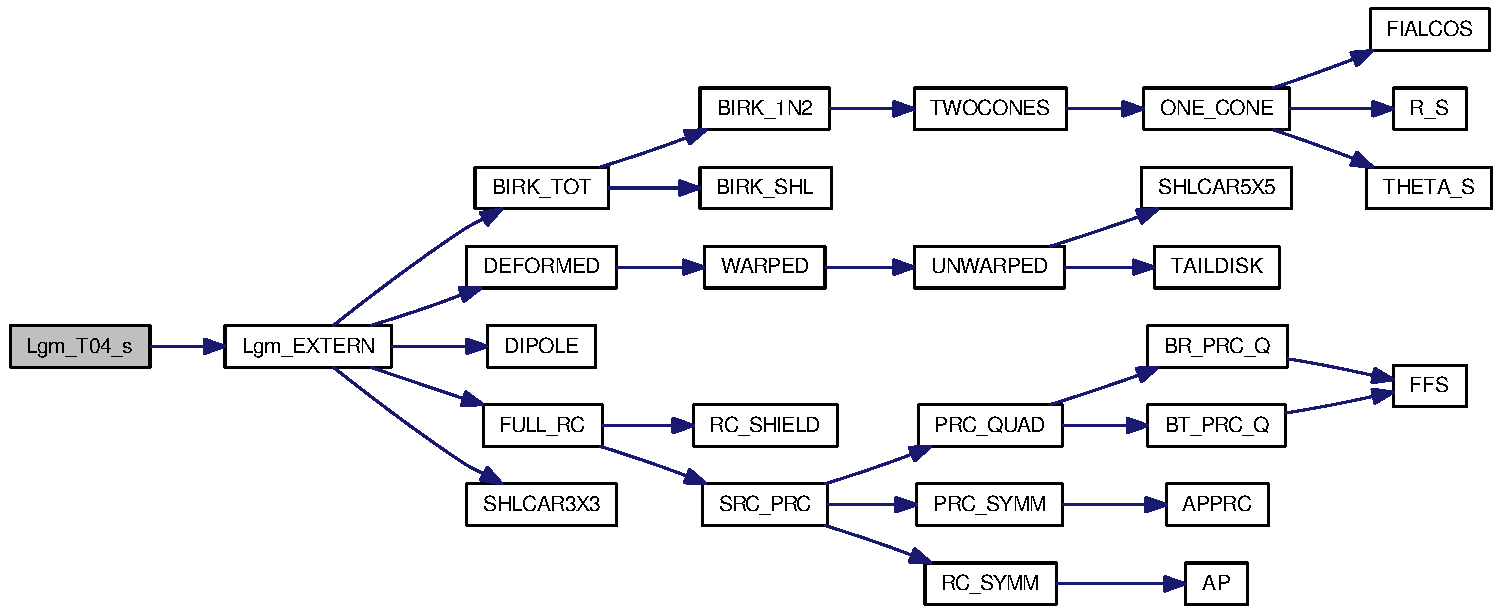
\includegraphics[width=378pt]{_tsyg2004_8c_54ecb238c46c4acfe5e022e19cc326ec_cgraph}
\end{center}
\end{figure}


Here is the caller graph for this function:\nopagebreak
\begin{figure}[H]
\begin{center}
\leavevmode
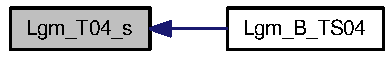
\includegraphics[width=112pt]{_tsyg2004_8c_54ecb238c46c4acfe5e022e19cc326ec_icgraph}
\end{center}
\end{figure}


\subsection{Variable Documentation}
\hypertarget{_tsyg2004_8c_5b35fcda1a15310fa7b7e3e242431de3}{
\index{Tsyg2004.c@{Tsyg2004.c}!sin\_\-psi@{sin\_\-psi}}
\index{sin\_\-psi@{sin\_\-psi}!Tsyg2004.c@{Tsyg2004.c}}
\subsubsection[{sin\_\-psi}]{\setlength{\rightskip}{0pt plus 5cm}double {\bf sin\_\-psi}}}
\label{_tsyg2004_8c_5b35fcda1a15310fa7b7e3e242431de3}




Definition at line 108 of file Tsyg2004.c.\hypertarget{_tsyg2004_8c_98e0e08bb8a65f90813e5adb482aeb2c}{
\index{Tsyg2004.c@{Tsyg2004.c}!cos\_\-psi@{cos\_\-psi}}
\index{cos\_\-psi@{cos\_\-psi}!Tsyg2004.c@{Tsyg2004.c}}
\subsubsection[{cos\_\-psi}]{\setlength{\rightskip}{0pt plus 5cm}double {\bf cos\_\-psi}}}
\label{_tsyg2004_8c_98e0e08bb8a65f90813e5adb482aeb2c}




Definition at line 108 of file Tsyg2004.c.